\documentclass[11pt]{article}

% ---------- Packages ----------
\usepackage[margin=1in]{geometry}
\usepackage{amsmath,amsthm,graphicx,enumitem,amssymb}
\usepackage{mathtools}
\usepackage{physics}        % derivatives, bras/kets, etc.
\usepackage{siunitx}        % units
\usepackage{graphicx}       % figures
\usepackage{float}          % figure placement
\usepackage{booktabs}       % nice tables
\usepackage{enumitem}       % better lists
\usepackage{fancyhdr}       % header/footer
\usepackage{titlesec}       % section formatting
\usepackage{hyperref}       % links
\usepackage{tcolorbox}      % boxes for answers
\usepackage{listings}       % code (MATLAB, Python, etc.)
\usepackage{xcolor}
\usepackage{bbm}        % blackboard bold italic


% Define colors
\definecolor{codegreen}{rgb}{0,0.6,0}
\definecolor{codepurple}{rgb}{0.58,0,0.82}
\definecolor{backcolour}{rgb}{0.95,0.95,0.92}

% ---------- Hyperref Setup ----------
\hypersetup{
    colorlinks=true,
    linkcolor=blue,
    urlcolor=blue,
    citecolor=blue
}

% ---------- Header/Footer ----------
\pagestyle{fancy}
\fancyhf{}
\lhead{\textbf{\course}}
\rhead{\textbf{\assignment}}
\cfoot{\thepage}

% ---------- Custom Commands ----------
\newcommand{\course}{ASEN 6044}
\newcommand{\assignment}{Homework \#2}
\newcommand{\studentname}{Bijan Jourabchi}

\newcommand{\R}{\mathbb{R}}
\newcommand{\E}{\mathbb{E}}
\newcommand{\Var}{\mathrm{Var}}
\newcommand{\Cov}{\mathrm{Cov}}

% Boxed answer environment
\newtcolorbox{answerbox}{
    colback=gray!5,
    colframe=gray!50,
    title=Answer,
    fonttitle=\bfseries
}

% Problem section format
\titleformat{\section}{\large\bfseries}{Problem \thesection:}{0.5em}{}

% ---------- Code Style ----------
\lstset{
    basicstyle=\ttfamily\small,
    keywordstyle=\color{blue},
    commentstyle=\color{green!50!black},
    stringstyle=\color{orange},
    breaklines=true,
    frame=single
    extendedchars=true,
    literate={π}{{$\pi$}}1 {γ}{{$\gamma$}}1
}

% ---------- Document ----------
\begin{document}

% ---------- Title Block ----------
\begin{center}
    {\LARGE \textbf{\course}} \\[6pt]
    {\Large \assignment} \\[10pt]
    \studentname \\
\end{center}

\vspace{1em}
\hrule
\vspace{1em}


% =====================================================
\section{}

We are given a prior and measurement likelihood given by
\begin{align*}
    P(\theta) = \begin{cases}
        \alpha e^{-\alpha\theta} \quad \theta \geq 0 \\
        0 \quad \theta < 0
    \end{cases} \\
    P(y \mid \theta) = \frac{\theta^y e^{-\theta}}{y!} \quad y \in \mathbb{Z^+}
\end{align*}
From Bayes Rule, we know the posterior distribution is given by
\[
P(\theta \mid y) = \frac{P(y \mid \theta)P(\theta)}{P(y)}
\]
Where $P(y)$ is given by the marginalization of the joint distribution $P(\theta,y)$, that is
\[P(y) = \int_{-\infty}^\infty P(\theta, y) d\theta = \int_{-\infty}^\infty P(y \mid \theta)P(\theta) d\theta
= \int_{0}^\infty \alpha e^{-\alpha\theta} \frac{\theta^y e^{-\theta}}{y!} d\theta \]
Since we are given $y$, $P(y)$ is a constant and is not dependent on $\theta$. Thus, our posterior distribution will be 
proportional to the measurement likelihood times the prior.
\[
 P(\theta \mid y) \propto \alpha e^{-\alpha\theta} \frac{\theta^y e^{-\theta}}{y!} = \frac{\alpha \theta^y e^{-\theta(1+\alpha)}}{y!}
\] 
Recall the pdf of a gamma distribution:
\[
f(x) = \Gamma(\gamma,\beta) = \frac{\beta^{\gamma}x^{\gamma-1}e^{-\beta x}}{\Gamma(\gamma)}
\]
Where $\Gamma(\gamma)$ is the gamma function. For positive integers, the gamma function returns $\Gamma(n) = (n-1)!$. Since $y$ is a positive integer, it's clear that our posterior distribution is a gamma distribution with parameters $\gamma = y+1$ and $\beta = \alpha+1$.

\begin{enumerate}[label=\alph*)]
    \item 
    The MMSE estimate for our posterior distribution is the expected value of the distribution.
    \[
    \hat{\theta}_{MMSE} = \mathbb{E}[P(\theta\mid y)]
    \]

    For a gamma distribution, the expected value is given by $\mathbb{E}[\Gamma(\gamma,\beta)] = \frac{\gamma}{\beta}$. Thus, the MMSE estimate
    for our posterior distribution is
    \begin{align*}
        \boxed{\hat{\theta}_{MMSE} = \frac{y+1}{\alpha+1}}
    \end{align*}
    \item
    The MAP estimate for our posterior distribution is the maximum value of our posterior. We can find the maximum
    by taking the derivative of our posterior with respect to $\theta$ and setting equal to 0.
    \begin{align*}
        & \frac{d}{d\theta} \Big[\frac{\alpha \theta^y e^{-\theta(1+\alpha)}}{y!}\Big] = \frac{\alpha[y\theta^{y-1}e^{-\theta(1+\alpha)}-(1+\alpha)e^{-\theta(1+\alpha)}\theta^y]}{y!} = 0 \\
        & [y\theta^{y-1}-(\alpha+1)\theta^y]e^{-\theta(1+\alpha)} = 0 \to (\alpha+1)\theta^y = y\theta^{y-1} \\
        & \alpha + 1 = y\theta^{-1} \to \boxed{\hat{\theta}_{MAP} = \frac{y}{\alpha+1}}
    \end{align*}
\end{enumerate}

% =====================================================
\section{}

We are given that a continous random variable $\theta$ is uniformly distributed on the interval $[0,1]$, and that measurements are given by
$y = \theta + n$ where $n$'s distribution is given as
\[
P(n) = \begin{cases}
    e^{-n} \quad n \geq 0 \\
    0 \quad n < 0
\end{cases}
\]
From the following pdf, we can derive our measurement likelihood $P(y\mid\theta)$. Since our noise is additive, we have $n = y-\theta$. Plugging this into $P(n)$ we have
\[
P(y\mid\theta) = P(y-\theta) = \begin{cases}
    e^{-y+\theta} \quad y \geq \theta \\
    0 \quad y < \theta
\end{cases}
\]
For a fixed observation y, this is identical to the measurement likelihood, $P(y\mid\theta)$. Applying Bayes Rule, we can derive an expression for our posterior.
\begin{align*}
    P(\theta \mid y) = \frac{P(y\mid\theta)P(\theta)}{\int_{-\infty}^{\infty}P(y\mid\theta)P(\theta) d\theta}
\end{align*}
The bounds on the posterior must be consistent with the constraints placed on the prior and likelihood. We know $\theta \in [0,1]$ and $y \geq \theta$.
Thus, we know our posterior estimate should be cut off at $\theta = 1$ is $y \geq 1$. However, if $y < 1$, we know that theta cannot be larger than $y$. Thus, an upper bound on our posterior distribution becomes
$u = \min(1,y)$. We can use this upper bound to solve for the normalizing integral in posterior expression.
\begin{align*}
    & \int_{-\infty}^{\infty}P(y\mid\theta)P(\theta) d\theta = \int_{0}^{u}P(y\mid\theta)P(\theta) d\theta = \int_{0}^{u}e^{-y}e^{\theta} d\theta \\
    & = e^{-y}[e^u - 1]
\end{align*}
And out posterior becomes 
\[
    P(\theta \mid y) = \begin{cases}
        \frac{e^\theta}{e^u-1} \quad 0 \leq \theta \leq u \\ 
        0 \quad \mathrm{o.w}
    \end{cases} u = \min(1,y)
\]
\begin{enumerate}[label=\alph*)]
    \item $\hat{\theta}_{MMSE} = \mathbb{E}[P(\theta\mid y)]$ by definition. Thus, we can evaluate the expected value to receive an expression for $\hat{\theta}_{MMSE}$.
    \begin{align*}
        \mathbb{E}[P(\theta\mid y)] &= \int_0^u \theta \frac{e^\theta}{e^u-1} d\theta = \frac{1}{e^u-1}\Big[ \eval{\theta e^\theta}_{0}^{u} - \int_0^u e^\theta d\theta\Big] \\
        & = \frac{1}{e^u-1} \Big[ue^u - e^u+1\Big] = \frac{ue^u - e^u+1}{e^u-1}
    \end{align*}
    Thus $\hat{\theta}_{MMSE} = \mathbb{E}[P(\theta\mid y)] = \boxed{\frac{ue^u - e^u+1}{e^u-1}}$
    \item
        By taking the derivative of our posterior we can derive an expression for $\hat{\theta}_{MAP}$.
        \[
            \frac{d}{d\theta} \Big[\frac{e^\theta}{e^u-1}\Big] = \frac{e^\theta}{e^u-1}
        \]
        Since this function is monotonic increasing, is maximum must lie at the end of the interval. Thus, $\boxed{\hat{\theta}_{MAP} = \min(u,1)}$.
\end{enumerate}
\section{}

\begin{enumerate}[label=\alph*)]
    \item
    \begin{figure}[h]
        \centering
            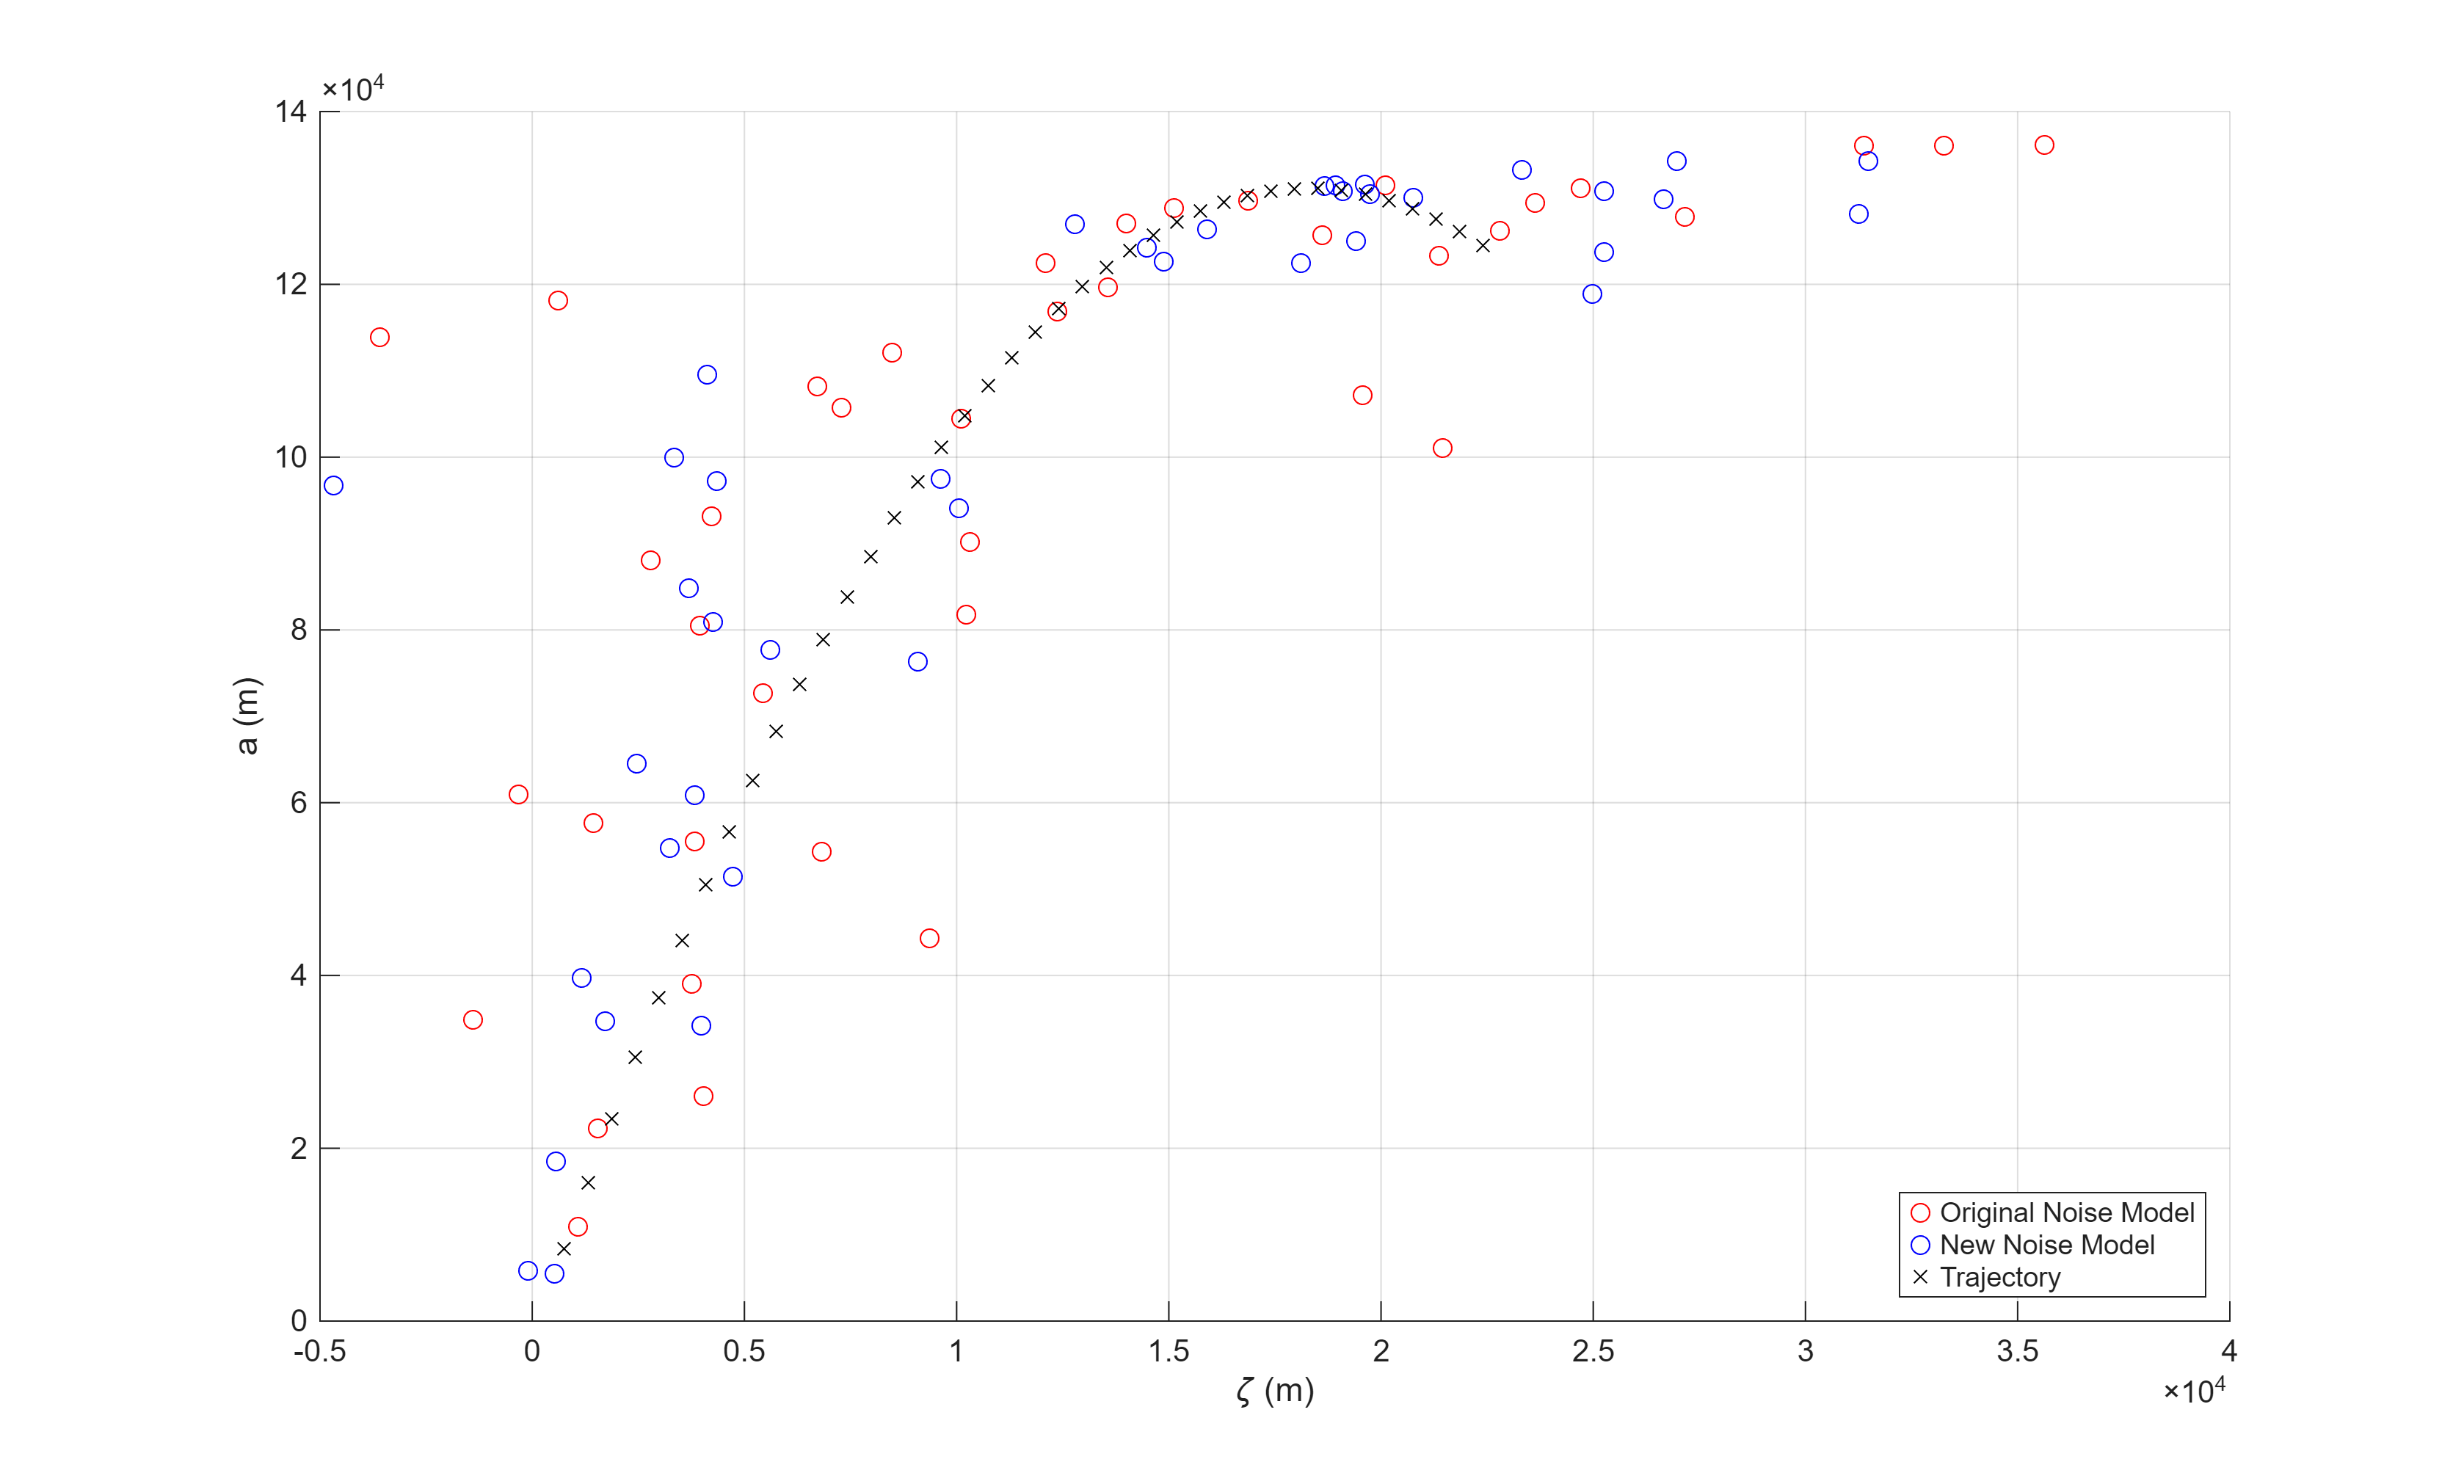
\includegraphics[width=\textwidth, height=0.75\textheight, keepaspectratio]{Figures/missile_measurments.png}
        \caption{Comparison of Old and New Noisy measurements}
        \label{fig:measurements}
    \end{figure}

    From Figure \ref{fig:measurements} we see generally that the measurements from the new noisy range model draw out a similar shape
    to that of the old range model. Without any prior knowledge regarding the problem, it even appears that both sets of measurements have the same noise model.
    \item
    \begin{figure}[h]
        \centering
            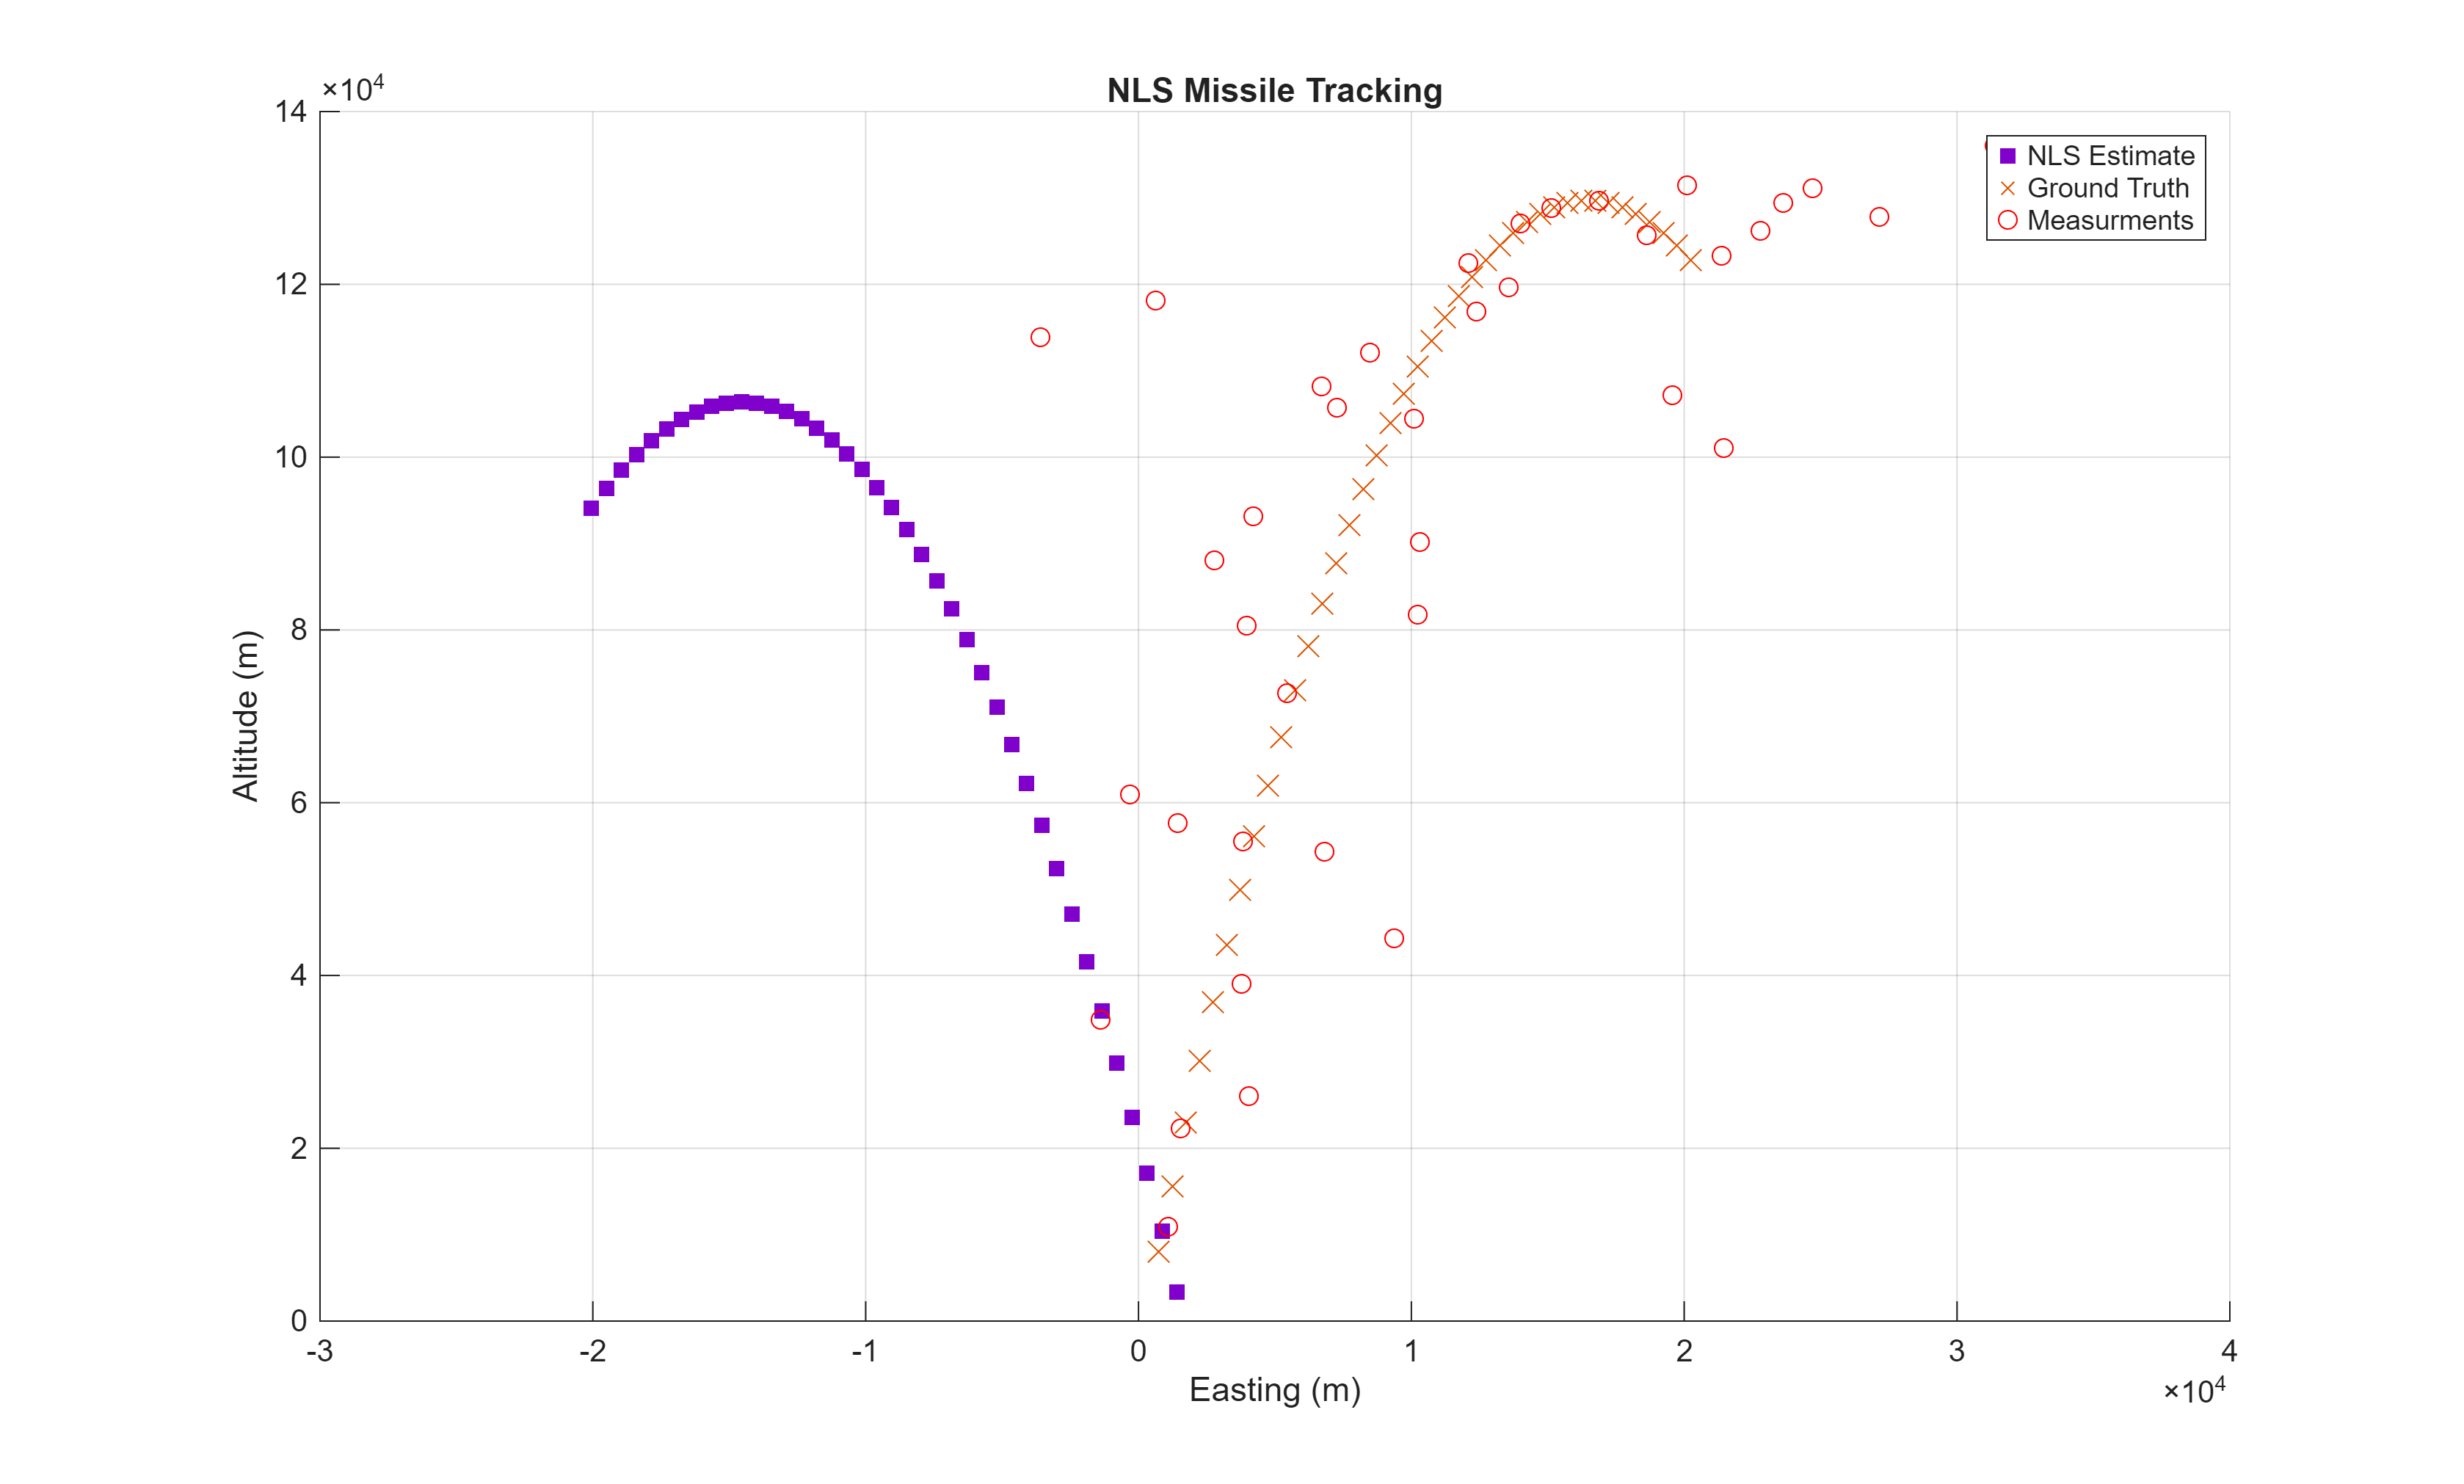
\includegraphics[width=\textwidth, height=0.75\textheight, keepaspectratio]{Figures/NLS_estimate.png}
        \caption{NLS Estimated Trajectory Under New Noise Model}
        \label{fig:NLS}
    \end{figure}

    \begin{figure}[h]
        \centering
        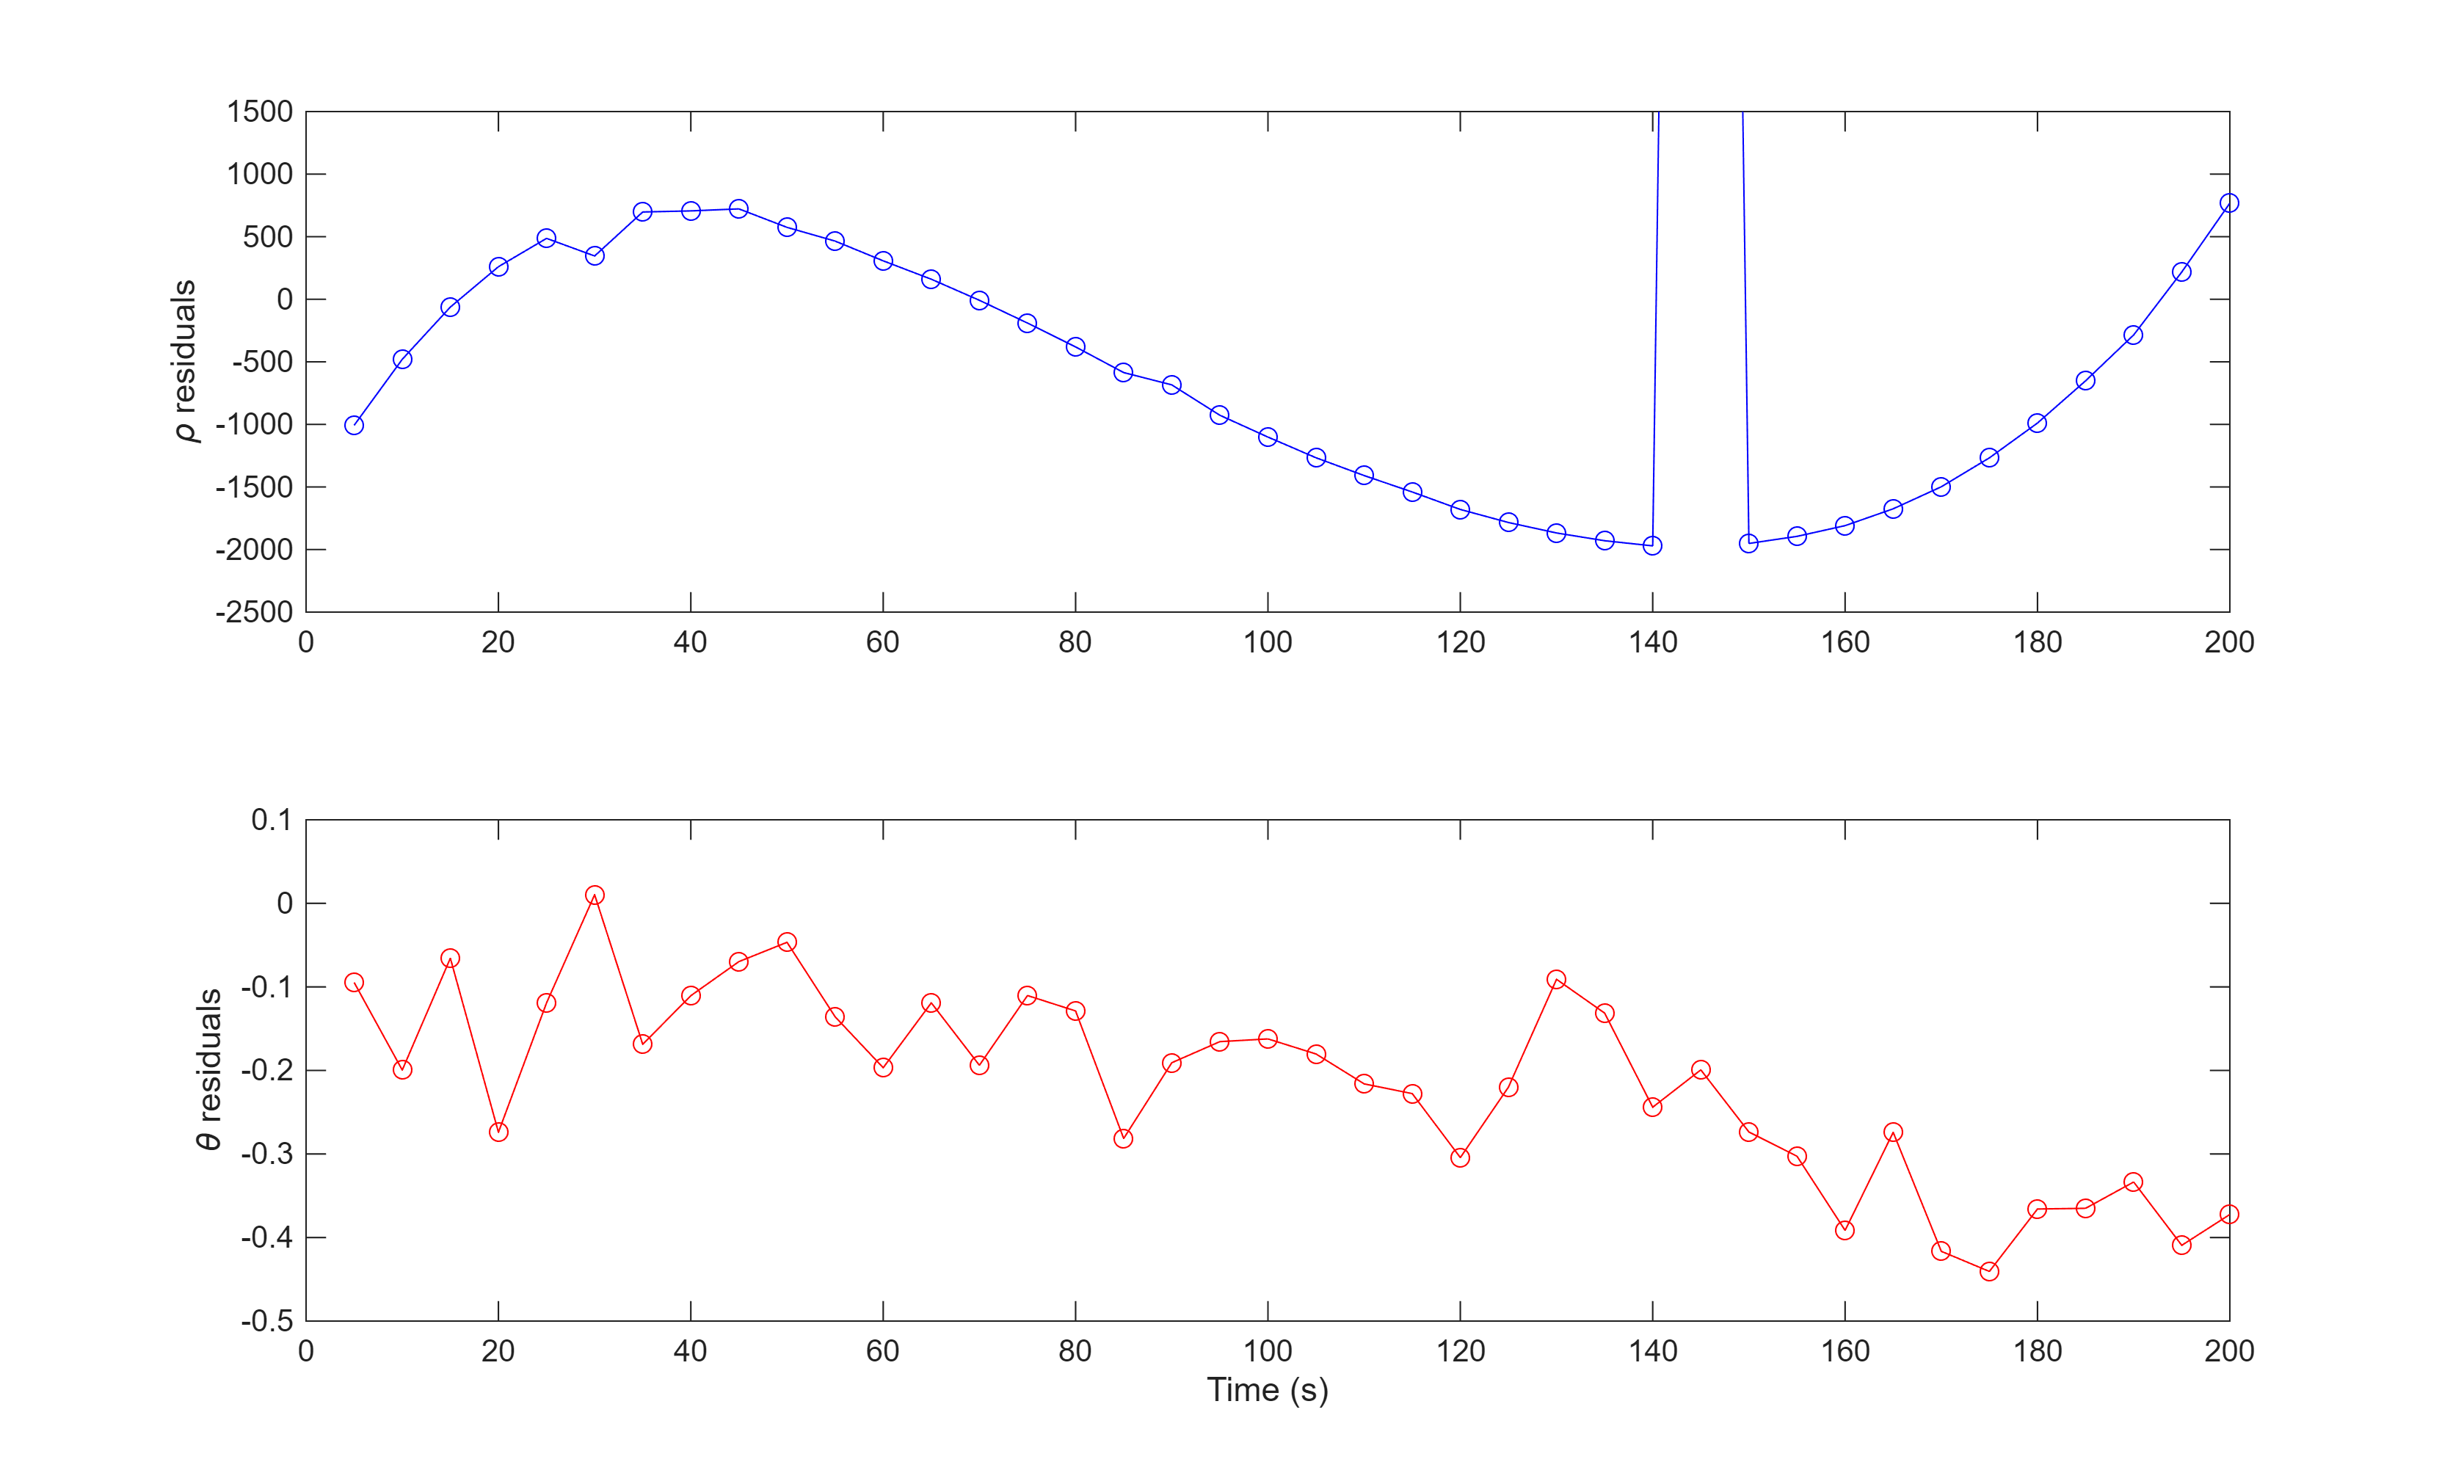
\includegraphics[width=\textwidth,height=0.75\textheight, keepaspectratio]{Figures/NLS_estimate_Res.png}
        \caption{NLS measurement Residuals with $\rho$ Outlier Removed}
        \label{fig:NLSres}
    \end{figure}

    Using the NLS batch estimation code from HW 1 and with an initial $x_{0} = [10 \ 30 \ 230 \ 100]^T$ we get the results seen in figure \ref{fig:NLS}. As opposed to HW1, NLS does not work well for the new proposed noise model.
    This is almost certainly due to the fact that a Student's t-distribution with $\nu = \frac{1}{2}$ does not have a well-defined variance. The non-Gaussian sensor noise present means the lease-square cost function is not appropriate for this type of problem.
    This is due to the new Student's t-distribution having higher order moments that our model is not capturing in $R$. Thus, the algorithm is not able to make sense of the data is seeing. This is also seen in figure \ref{fig:NLSres} where the range residuals in particular are very large.
    NLS converged on an estimate of $\hat{x}_{0,NLS} = [1.96 \times 10^3 \  -110.04 \  -3.83\times 10^3 \ 1.47 \times 10^3]^T$ giving NLS an error of $[-1.72\times 10^3 \ 210 \ 4 \times 10^3 \ 123.6]^T$. We can also find a resulting covariance, however due to the large residual the covariance estimate is unreliable.
    \[
    P(\hat{x}_{0,NLS}) = \begin{bmatrix}
        37.8	& -0.86	& 44.2	& -0.87 \\
    -0.86	& 0.051	& -0.314	& 0.045 \\
    44.2	& -0.314	& 98.5	& -0.69 \\
    -0.874 & 0.045	& -0.69	& 0.04
    \end{bmatrix}
    \] 
    \item 
    
    The negative log-likelihood function, $\mathcal{L}(x_0;Y_{1:N}) = J_{NLL}$ is defined as the negative logarithm of the measurement likelihood functions, that is
    \[
        J_{NLL} = -\log(P(Y_{1:N} \mid x_0))
    \]

    To derive an expression for $P(Y_{1:N} \mid x_0)$, we look at the given measurement model:

    \begin{align}
        \rho_k = \sqrt{(L-\xi(t_k))^2 + (a(t_k))^2} + v_{r,k} \quad v_{r,k} \sim \mathcal{T}_{v_{r,k}} \Big(0,\nu = \frac{1}{2}\Big) \label{eq:range}\\
        \theta_k = \arctan(\frac{a(t_k)}{L-\xi(t_k)}) + v_{b,k} \quad v_{b,k} \sim \mathcal{N}_{v_{b,k}} \Big(0,\sigma_b^2 = 0.005\Big)
        \label{eq:bearing}
    \end{align}
    
    Where $v_{r,k}$ and $v_{b,k}$ are the range and bearing noise respectively. To derive the measurement likelihood $P(Y_{1:N} \mid x_0)$ we assume that the measurements are conditionally independent 
    given $x_0$, that is $P(Y_{1:N} \mid x_0) = \prod_{k=1}^{N}P(y_k \mid x_0)$. We also assume that the range and bearing measurements are independent of each other, so our expression further simplifies to the following:

    \begin{align}
        P(Y_{1:N} \mid x_0) = \prod_{k=1}^{N}  P(\rho_k \mid x_0) P(\theta_k \mid x_0)
        \label{eq:likelihood}
    \end{align}


    Since our noise is additive, solving for the respective probabilities is fairly straightforward. From (\ref{eq:range}) we can derive $P(\rho_k \mid x_0)$ as follows:

    \begin{align*}
        v_{r,k} &= \rho_k - \sqrt{(L-\xi(t_k))^2 + (a(t_k))^2} \\
        P(v_{r,k}) &= \frac{\Gamma(\frac{\nu + 1}{2})}{\Gamma(\frac{\nu}{2})\sqrt{\nu\pi}}\Big(1+\frac{v_{r,k}^2}{\nu} \Big)^{-\frac{\nu+1}{2}}
    \end{align*}

    Substituting for $v_{r,k}$ we get the following expression in terms of our initial conditions. 
    \begin{align}
        P(\rho_k \mid x_0) &= \frac{\Gamma(\frac{\nu + 1}{2})}{\Gamma(\frac{\nu}{2})\sqrt{\nu\pi}}\Big(1+\frac{(\rho_k - \sqrt{(L-\xi_0 - \dot{\xi_0}t_k)^2 + (a_0 + \dot{a_0}t_k - 0.5gt_k^2)})}{\nu} \Big)^{-\frac{\nu+1}{2}}
        \label{eq:Pr}
    \end{align}
    We can follow a similar process to derive $P(\theta_k \mid x_0)$.
    \begin{align*}
        v_{b,k} = \theta_k - \arctan(\frac{a(t_k)}{\xi(t_k)}) \\
        P(v_{b,k}) = \frac{1}{\sigma_b\sqrt{2\pi}}\exp{\frac{-1}{2\sigma_b^2}v_{b,k}^2}
    \end{align*}
    \begin{align}
        P(\theta_k \mid x_0) &= \frac{1}{\sigma_b \sqrt{2\pi}} \exp{\frac{-\Big[\theta_k-\arctan(\frac{a_0+\dot{a_0}t_k-0.5gt_k^2}{L-\xi_0-\dot{\xi_0}t_k})\Big]^2}{2\sigma_b^2}}
        \label{eq:Pb}
    \end{align}

    Substituting (\ref{eq:Pb}) and (\ref{eq:Pr}) into (\ref{eq:likelihood}) and taking the negative logarithm
    we receive the following expression for our negative log likelihood function:
    \begin{equation}
        \begin{split}
            \mathcal{L}(x_0;Y_{1:N}) &= - \sum_{k=1}^N \log[P(\rho_k \mid x_0) P(\theta_k \mid x_0)] \\
            &= - \sum_{k=1}^N \log(\frac{\Gamma(\frac{\nu + 1}{2})}{\Gamma(\frac{\nu}{2})\sqrt{\nu\pi}}\frac{1}{\sigma_b \sqrt{2\pi}}) 
            \\ &\quad -\sum_{k=1}^N -\frac{\nu+1}{2}\log(1+\frac{(\rho_k - \sqrt{(L-\xi_0 - \dot{\xi_0}t_k)^2 + (a_0 + \dot{a_0}t_k - 0.5gt_k^2)})}{\nu} ) \\
            &\quad -\sum_{k=1}^N \frac{-\Big[\theta_k-\arctan(\frac{a_0+\dot{a_0}t_k-0.5gt_k^2}{L-\xi_0-\dot{\xi_0}t_k})\Big]^2}{2\sigma_b^2}
        \end{split}
        \label{eq:JNLL}
    \end{equation}

    Both the NLL and NLS cost functions seek to find an $x_0$ that minimizes the cost function given observations $Y_{1:N}$, however they each approach the problem differently.
    NLS is defined to minimize the sum of the squared residuals, while maximum likelihood tries to find the $x_0$ which makes `the most sense' given all the observations. Both assume the measurement noise characteristics 
    are known, NLS uses a least squares cost function, meaning we only consider the 1st/2nd order moments. As we have seen with the Student's-t distribution, this does not accurately capture higher order moments. Maximum likelihood is robust to non-Gaussian
    sensor noise unlike the least-squares cost function we have selected for NLS. 
    \item
    In order to minimize (\ref{eq:JNLL}), we take the gradient with respect to $x_0$, or \(\nabla_{x_0}\mathcal{L}(x_0;Y_{1:N})\), where
    \begin{align*} 
        \nabla_{x_0} = \begin{bmatrix}
            \frac{\partial}{\partial \xi_0} \\
            \frac{\partial}{\partial \dot{\xi_0}} \\
            \frac{\partial}{\partial a_0} \\
            \frac{\partial}{\partial \dot{a_0}}
        \end{bmatrix}
    \end{align*}

\begin{align*}
    \nabla_{x_0}\mathcal{L}(x_0;Y_{1:N}) = -\nabla_{x_0} \sum_{k=1}^N \log[P(\rho_k \mid x_0) P(\theta_k \mid x_0)]
\end{align*}

It's easy to show that the expression simplifies to the following, where the constant terms evaluate to zero.
\begin{equation}
    \begin{split}
        &= -\nabla_{x_0}\Bigg[\frac{-\nu+1}{2}\log\Bigg(1+ \frac{\Big(\rho_k - \sqrt{(L-\xi_0 - \dot{\xi_0}t_k)^2 + (a_0 + \dot{a_0} - 0.5gt_k^2)^2} \ \Big)^2}{\nu}\Bigg)\Bigg] \\
        &\quad -\nabla_{x_0}\Big[\frac{-1}{2}\Big[\frac{\theta_k - \arctan(\frac{a_0 + \dot{a_0}t_k - 0.5gt_k^2}{L-\xi_0-\dot{\xi_0}t_k})}{\sigma_b}\Big]^2\Big]
    \end{split}
    \label{eq:gradient_nll}
\end{equation}

Equation (\ref{eq:gradient_nll}) consists of two gradient terms to evaluate. Starting with the first term, we can take each partial derivative independently and stack the result into a vector:

\[
\nabla_{x_0}\Bigg[\frac{-\nu+1}{2}\log\Bigg(1+ \frac{\Big(\rho_k - \sqrt{(L-\xi_0 - \dot{\xi_0}t_k)^2 + (a_0 + \dot{a_0} - 0.5gt_k^2)^2} \ \Big)^2}{\nu}\Bigg)\Bigg]
\]


\begin{align*}
    & \frac{\partial}{\partial \xi_0}\Bigg[\frac{-\nu+1}{2}\log\Bigg(1+ \frac{\Big(\rho_k - \sqrt{(L-\xi_0 - \dot{\xi_0}t_k)^2 + (a_0 + \dot{a_0} - 0.5gt_k^2)^2} \ \Big)^2}{\nu}\Bigg)\Bigg] \\
    & = \frac{-\nu + 1}{2} \frac{1}{\frac{(\rho_k - \sqrt{(L-\xi_0 - \dot{\xi_0}t_k)^2 + (a_0 + \dot{a_0}t - 0.5gt_k^2)^2})^2}{\nu} + 1} \frac{2}{\nu} (\rho_k - \sqrt{(L-\xi_0 - \dot{\xi_0}t_k)^2 + (a_0 + \dot{a_0}t - 0.5gt_k^2)^2}) \\
    & \frac{-1}{2\sqrt{(L-\xi_0 - \dot{\xi_0}t_k)^2 + (a_0 + \dot{a_0}t - 0.5gt_k^2)^2}} [-2(L-\xi_0 - \dot{\xi_0}t_k)]\\
    & = \frac{2(\rho_k - \sqrt{(L-\xi_0 - \dot{\xi_0})^2 + (a_0 + \dot{a_0}t - 0.5gt_k^2)^2})(L-\xi_0-\dot{\xi_0}t)}
    {(\Big(\rho - \sqrt{(L-\xi_0-\dot{\xi_0})^2 + (a_o + \dot{a_0}t-0.5gt^2)^2}\Big)^2 + \nu)\sqrt{(L-\xi_0-\dot{\xi_0})^2 + (a_o + \dot{a_0}t-0.5gt^2)^2}} 
\end{align*}

The remaining derivatives follow in a very similar fashion.

\begin{align*}
    &\frac{\partial}{\partial \dot{\xi_0}}\Bigg[\frac{-\nu+1}{2}\log\Bigg(1+ \frac{\Big(\rho_k - \sqrt{(L-\xi_0 - \dot{\xi_0}t_k)^2 + (a_0 + \dot{a_0} - 0.5gt_k^2)^2} \ \Big)^2}{\nu}\Bigg)\Bigg] \\
    &= \frac{2t(\rho_k - \sqrt{(L-\xi_0 - \dot{\xi_0})^2 + (a_0 + \dot{a_0}t - 0.5gt_k^2)^2})(L-\xi_0-\dot{\xi_0}t)}
    {(\Big(\rho - \sqrt{(L-\xi_0-\dot{\xi_0})^2 + (a_o + \dot{a_0}t-0.5gt^2)^2}\Big)^2 + \nu)\sqrt{(L-\xi_0-\dot{\xi_0})^2 + (a_o + \dot{a_0}t-0.5gt^2)^2}} 
\end{align*}

\begin{align*}
    &\frac{\partial}{\partial a_0}\Bigg[\frac{-\nu+1}{2}\log\Bigg(1+ \frac{\Big(\rho_k - \sqrt{(L-\xi_0 - \dot{\xi_0}t_k)^2 + (a_0 + \dot{a_0} - 0.5gt_k^2)^2} \ \Big)^2}{\nu}\Bigg)\Bigg] \\
    &= \frac{-2(\rho_k - \sqrt{(L-\xi_0 - \dot{\xi_0})^2 + (a_0 + \dot{a_0}t - 0.5gt_k^2)^2})(a_0+\dot{a_0}t-0.5gt^2)}
    {(\Big(\rho - \sqrt{(L-\xi_0-\dot{\xi_0})^2 + (a_o + \dot{a_0}t-0.5gt^2)^2}\Big)^2 + \nu)\sqrt{(L-\xi_0-\dot{\xi_0})^2 + (a_o + \dot{a_0}t-0.5gt^2)^2}} 
\end{align*}

\begin{align*}
    &\frac{\partial}{\partial \dot{a_0}}\Bigg[\frac{-\nu+1}{2}\log\Bigg(1+ \frac{\Big(\rho_k - \sqrt{(L-\xi_0 - \dot{\xi_0}t_k)^2 + (a_0 + \dot{a_0} - 0.5gt_k^2)^2} \ \Big)^2}{\nu}\Bigg)\Bigg] \\
    &= \frac{-2t(\rho_k - \sqrt{(L-\xi_0 - \dot{\xi_0})^2 + (a_0 + \dot{a_0}t - 0.5gt_k^2)^2})(a_0+\dot{a_0}t-0.5gt^2)}
    {(\Big(\rho - \sqrt{(L-\xi_0-\dot{\xi_0})^2 + (a_o + \dot{a_0}t-0.5gt^2)^2}\Big)^2 + \nu)\sqrt{(L-\xi_0-\dot{\xi_0})^2 + (a_o + \dot{a_0}t-0.5gt^2)^2}} 
\end{align*}

Therefore, 
\begin{align*}
    \nabla_{x_0}\Bigg[\frac{-\nu+1}{2}\log\Bigg(1+ \frac{\Big(\rho_k - \sqrt{(L-\xi_0 - \dot{\xi_0}t_k)^2 + (a_0 + \dot{a_0} - 0.5gt_k^2)^2} \ \Big)^2}{\nu}\Bigg)\Bigg] \\
\end{align*}
\begin{align}
    &= \frac{-\nu+1}{2} \begin{bmatrix}
        \frac{2(\rho_k - \sqrt{(L-\xi_0 - \dot{\xi_0})^2 + (a_0 + \dot{a_0}t - 0.5gt_k^2)^2})(L-\xi_0-\dot{\xi_0}t)}
    {\Big(\Big(\rho - \sqrt{(L-\xi_0-\dot{\xi_0})^2 + (a_o + \dot{a_0}t-0.5gt^2)^2}\Big)^2 + \nu\Big)\sqrt{(L-\xi_0-\dot{\xi_0})^2 + (a_o + \dot{a_0}t-0.5gt^2)^2}}  \\
    \frac{2t(\rho_k - \sqrt{(L-\xi_0 - \dot{\xi_0})^2 + (a_0 + \dot{a_0}t - 0.5gt_k^2)^2})(L-\xi_0-\dot{\xi_0}t)}
    {\Big(\Big(\rho - \sqrt{(L-\xi_0-\dot{\xi_0})^2 + (a_o + \dot{a_0}t-0.5gt^2)^2}\Big)^2 + \nu\Big)\sqrt{(L-\xi_0-\dot{\xi_0})^2 + (a_o + \dot{a_0}t-0.5gt^2)^2}} \\
    \frac{-2(\rho_k - \sqrt{(L-\xi_0 - \dot{\xi_0})^2 + (a_0 + \dot{a_0}t - 0.5gt_k^2)^2})(a_0+\dot{a_0}t-0.5gt^2)}
    {\Big(\Big(\rho - \sqrt{(L-\xi_0-\dot{\xi_0})^2 + (a_o + \dot{a_0}t-0.5gt^2)^2}\Big)^2 + \nu\Big)\sqrt{(L-\xi_0-\dot{\xi_0})^2 + (a_o + \dot{a_0}t-0.5gt^2)^2}} \\
    \frac{-2t(\rho_k - \sqrt{(L-\xi_0 - \dot{\xi_0})^2 + (a_0 + \dot{a_0}t - 0.5gt_k^2)^2})(a_0+\dot{a_0}t-0.5gt^2)}
    {\Big(\Big(\rho - \sqrt{(L-\xi_0-\dot{\xi_0})^2 + (a_o + \dot{a_0}t-0.5gt^2)^2}\Big)^2 + \nu\Big)\sqrt{(L-\xi_0-\dot{\xi_0})^2 + (a_o + \dot{a_0}t-0.5gt^2)^2}} 
    \end{bmatrix}
    \label{eq:Grad1}
\end{align}

We will follow a similar process for the second gradient term.

\begin{align*}
    &\nabla_{x_0}\Big[\frac{-1}{2}\Big[\frac{\theta_k - \arctan(\frac{a_0 + \dot{a_0}t_k - 0.5gt_k^2}{L-\xi_0-\dot{\xi_0}t_k})}{\sigma_b}\Big]^2\Big]
    = \frac{-1}{2\sigma_b^2} \nabla_{x_0} \Big[\theta_k - \arctan(\frac{a_0 + \dot{a_0}t_k - 0.5gt_k^2}{L-\xi_0-\dot{\xi_0}t_k})\Big]^2
\end{align*}
\begin{align*}
    &\frac{\partial}{\partial \xi_0} \Big[\theta_k - \arctan(\frac{a_0 + \dot{a_0}t_k - 0.5gt_k^2}{L-\xi_0-\dot{\xi_0}t_k})\Big]^2 
    = \frac{-2t[\theta_k - \arctan(\frac{a_0 + \dot{a_0}t_k - 0.5gt_k^2}{L-\xi_0-\dot{\xi_0}t_k})](a_o+\dot{a_0}t_k-0.5gt_k^2)}{([\frac{a_0 + \dot{a_0}t_k - 0.5gt_k^2}{L-\xi_0-\dot{\xi_0}t_k}]^2 + 1)(L-\xi_0-\dot{\xi_0}t_k)^2}
\end{align*}
\begin{align*}
    &\frac{\partial}{\partial \dot{\xi_0}} \Big[\theta_k - \arctan(\frac{a_0 + \dot{a_0}t_k - 0.5gt_k^2}{L-\xi_0-\dot{\xi_0}t_k})\Big]^2 
    = \frac{-2[\theta_k - \arctan(\frac{a_0 + \dot{a_0}t_k - 0.5gt_k^2}{L-\xi_0-\dot{\xi_0}t_k})](a_o+\dot{a_0}t_k-0.5gt_k^2)}{([\frac{a_0 + \dot{a_0}t_k - 0.5gt_k^2}{L-\xi_0-\dot{\xi_0}t_k}]^2 + 1)(L-\xi_0-\dot{\xi_0}t_k)^2}
\end{align*}
\begin{align*}
    &\frac{\partial}{\partial a_0} \Big[\theta_k - \arctan(\frac{a_0 + \dot{a_0}t_k - 0.5gt_k^2}{L-\xi_0-\dot{\xi_0}t_k})\Big]^2 
    = \frac{-2[\theta_k - \arctan(\frac{a_0 + \dot{a_0}t_k - 0.5gt_k^2}{L-\xi_0-\dot{\xi_0}t_k})]}{([\frac{a_0 + \dot{a_0}t_k - 0.5gt_k^2}{L-\xi_0-\dot{\xi_0}t_k}]^2 + 1)(L-\xi_0-\dot{\xi_0}t_k)}
\end{align*}
\begin{align*}
    &\frac{\partial}{\partial \dot{a_0}} \Big[\theta_k - \arctan(\frac{a_0 + \dot{a_0}t_k - 0.5gt_k^2}{L-\xi_0-\dot{\xi_0}t_k})\Big]^2
    = \frac{-2t[\theta_k - \arctan(\frac{a_0 + \dot{a_0}t_k - 0.5gt_k^2}{L-\xi_0-\dot{\xi_0}t_k})]}{([\frac{a_0 + \dot{a_0}t_k - 0.5gt_k^2}{L-\xi_0-\dot{\xi_0}t_k}]^2 + 1)(L-\xi_0-\dot{\xi_0}t_k)}
\end{align*}
\newpage
Therefore,

\begin{align}
    \nabla_{x_0}\Big[\frac{-1}{2}\Big[\frac{\theta_k - \arctan(\frac{a_0 + \dot{a_0}t_k - 0.5gt_k^2}{L-\xi_0-\dot{\xi_0}t_k})}{\sigma_b}\Big]^2\Big]
    = \frac{-1}{2\sigma_b^2} \begin{bmatrix}
        \frac{-2[\theta_k - \arctan(\frac{a_0 + \dot{a_0}t_k - 0.5gt_k^2}{L-\xi_0-\dot{\xi_0}t_k})](a_o+\dot{a_0}t_k-0.5gt_k^2)}{([\frac{a_0 + \dot{a_0}t_k - 0.5gt_k^2}{L-\xi_0-\dot{\xi_0}t_k}]^2 + 1)(L-\xi_0-\dot{\xi_0}t_k)^2} \\
        \frac{-2t[\theta_k - \arctan(\frac{a_0 + \dot{a_0}t_k - 0.5gt_k^2}{L-\xi_0-\dot{\xi_0}t_k})](a_o+\dot{a_0}t_k-0.5gt_k^2)}{([\frac{a_0 + \dot{a_0}t_k - 0.5gt_k^2}{L-\xi_0-\dot{\xi_0}t_k}]^2 + 1)(L-\xi_0-\dot{\xi_0}t_k)^2} \\
        \frac{-2[\theta_k - \arctan(\frac{a_0 + \dot{a_0}t_k - 0.5gt_k^2}{L-\xi_0-\dot{\xi_0}t_k})]}{([\frac{a_0 + \dot{a_0}t_k - 0.5gt_k^2}{L-\xi_0-\dot{\xi_0}t_k}]^2 + 1)(L-\xi_0-\dot{\xi_0}t_k)} \\
        \frac{-2t[\theta_k - \arctan(\frac{a_0 + \dot{a_0}t_k - 0.5gt_k^2}{L-\xi_0-\dot{\xi_0}t_k})]}{([\frac{a_0 + \dot{a_0}t_k - 0.5gt_k^2}{L-\xi_0-\dot{\xi_0}t_k}]^2 + 1)(L-\xi_0-\dot{\xi_0}t_k)}
    \end{bmatrix}
    \label{eq:Grad2}
\end{align}

Finally, we can substitute equations (\ref{eq:Grad1}) and (\ref{eq:Grad2}) into equation (\ref{eq:gradient_nll}) and we are left with an expression
for the gradient vector of $\mathcal{L}_{NLL}$

\begin{equation}
    \begin{split}
    \nabla_{x_0}\mathcal{L}(x_0;Y_{1:N}) &= \sum_{k=1}^N\Bigg[\frac{\nu-1}{2} \begin{bmatrix}
        \frac{2(\rho_k - \sqrt{(L-\xi_0 - \dot{\xi_0}t)^2 + (a_0 + \dot{a_0}t - 0.5gt_k^2)^2})(L-\xi_0-\dot{\xi_0}t)}
    {\Big(\Big(\rho - \sqrt{(L-\xi_0-\dot{\xi_0})^2 + (a_o + \dot{a_0}t-0.5gt^2)^2}\Big)^2 + \nu\Big)\sqrt{(L-\xi_0-\dot{\xi_0})^2 + (a_o + \dot{a_0}t-0.5gt^2)^2}}  \\
    \frac{2t(\rho_k - \sqrt{(L-\xi_0 - \dot{\xi_0}t)^2 + (a_0 + \dot{a_0}t - 0.5gt_k^2)^2})(L-\xi_0-\dot{\xi_0}t)}
    {\Big(\Big(\rho - \sqrt{(L-\xi_0-\dot{\xi_0})^2 + (a_o + \dot{a_0}t-0.5gt^2)^2}\Big)^2 + \nu\Big)\sqrt{(L-\xi_0-\dot{\xi_0})^2 + (a_o + \dot{a_0}t-0.5gt^2)^2}} \\
    \frac{-2(\rho_k - \sqrt{(L-\xi_0 - \dot{\xi_0}t)^2 + (a_0 + \dot{a_0}t - 0.5gt_k^2)^2})(a_0+\dot{a_0}t-0.5gt^2)}
    {\Big(\Big(\rho - \sqrt{(L-\xi_0-\dot{\xi_0})^2 + (a_o + \dot{a_0}t-0.5gt^2)^2}\Big)^2 + \nu\Big)\sqrt{(L-\xi_0-\dot{\xi_0})^2 + (a_o + \dot{a_0}t-0.5gt^2)^2}} \\
    \frac{-2t(\rho_k - \sqrt{(L-\xi_0 - \dot{\xi_0}t)^2 + (a_0 + \dot{a_0}t - 0.5gt_k^2)^2})(a_0+\dot{a_0}t-0.5gt^2)}
    {\Big(\Big(\rho - \sqrt{(L-\xi_0-\dot{\xi_0})^2 + (a_o + \dot{a_0}t-0.5gt^2)^2}\Big)^2 + \nu\Big)\sqrt{(L-\xi_0-\dot{\xi_0})^2 + (a_o + \dot{a_0}t-0.5gt^2)^2}} 
    \end{bmatrix} \\
    &+ \frac{1}{2\sigma_b^2} \begin{bmatrix}
        \frac{-2[\theta_k - \arctan(\frac{a_0 + \dot{a_0}t_k - 0.5gt_k^2}{L-\xi_0-\dot{\xi_0}t_k})](a_o+\dot{a_0}t_k-0.5gt_k^2)}{([\frac{a_0 + \dot{a_0}t_k - 0.5gt_k^2}{L-\xi_0-\dot{\xi_0}t_k}]^2 + 1)(L-\xi_0-\dot{\xi_0}t_k)^2} \\
        \frac{-2t[\theta_k - \arctan(\frac{a_0 + \dot{a_0}t_k - 0.5gt_k^2}{L-\xi_0-\dot{\xi_0}t_k})](a_o+\dot{a_0}t_k-0.5gt_k^2)}{([\frac{a_0 + \dot{a_0}t_k - 0.5gt_k^2}{L-\xi_0-\dot{\xi_0}t_k}]^2 + 1)(L-\xi_0-\dot{\xi_0}t_k)^2} \\
        \frac{-2[\theta_k - \arctan(\frac{a_0 + \dot{a_0}t_k - 0.5gt_k^2}{L-\xi_0-\dot{\xi_0}t_k})]}{([\frac{a_0 + \dot{a_0}t_k - 0.5gt_k^2}{L-\xi_0-\dot{\xi_0}t_k}]^2 + 1)(L-\xi_0-\dot{\xi_0}t_k)} \\
        \frac{-2t[\theta_k - \arctan(\frac{a_0 + \dot{a_0}t_k - 0.5gt_k^2}{L-\xi_0-\dot{\xi_0}t_k})]}{([\frac{a_0 + \dot{a_0}t_k - 0.5gt_k^2}{L-\xi_0-\dot{\xi_0}t_k}]^2 + 1)(L-\xi_0-\dot{\xi_0}t_k)}
    \end{bmatrix} \Bigg]
    \end{split}
    \label{eq:finalGrad}
\end{equation}
    \newpage
    \item
    \begin{figure}[h]
        \centering
        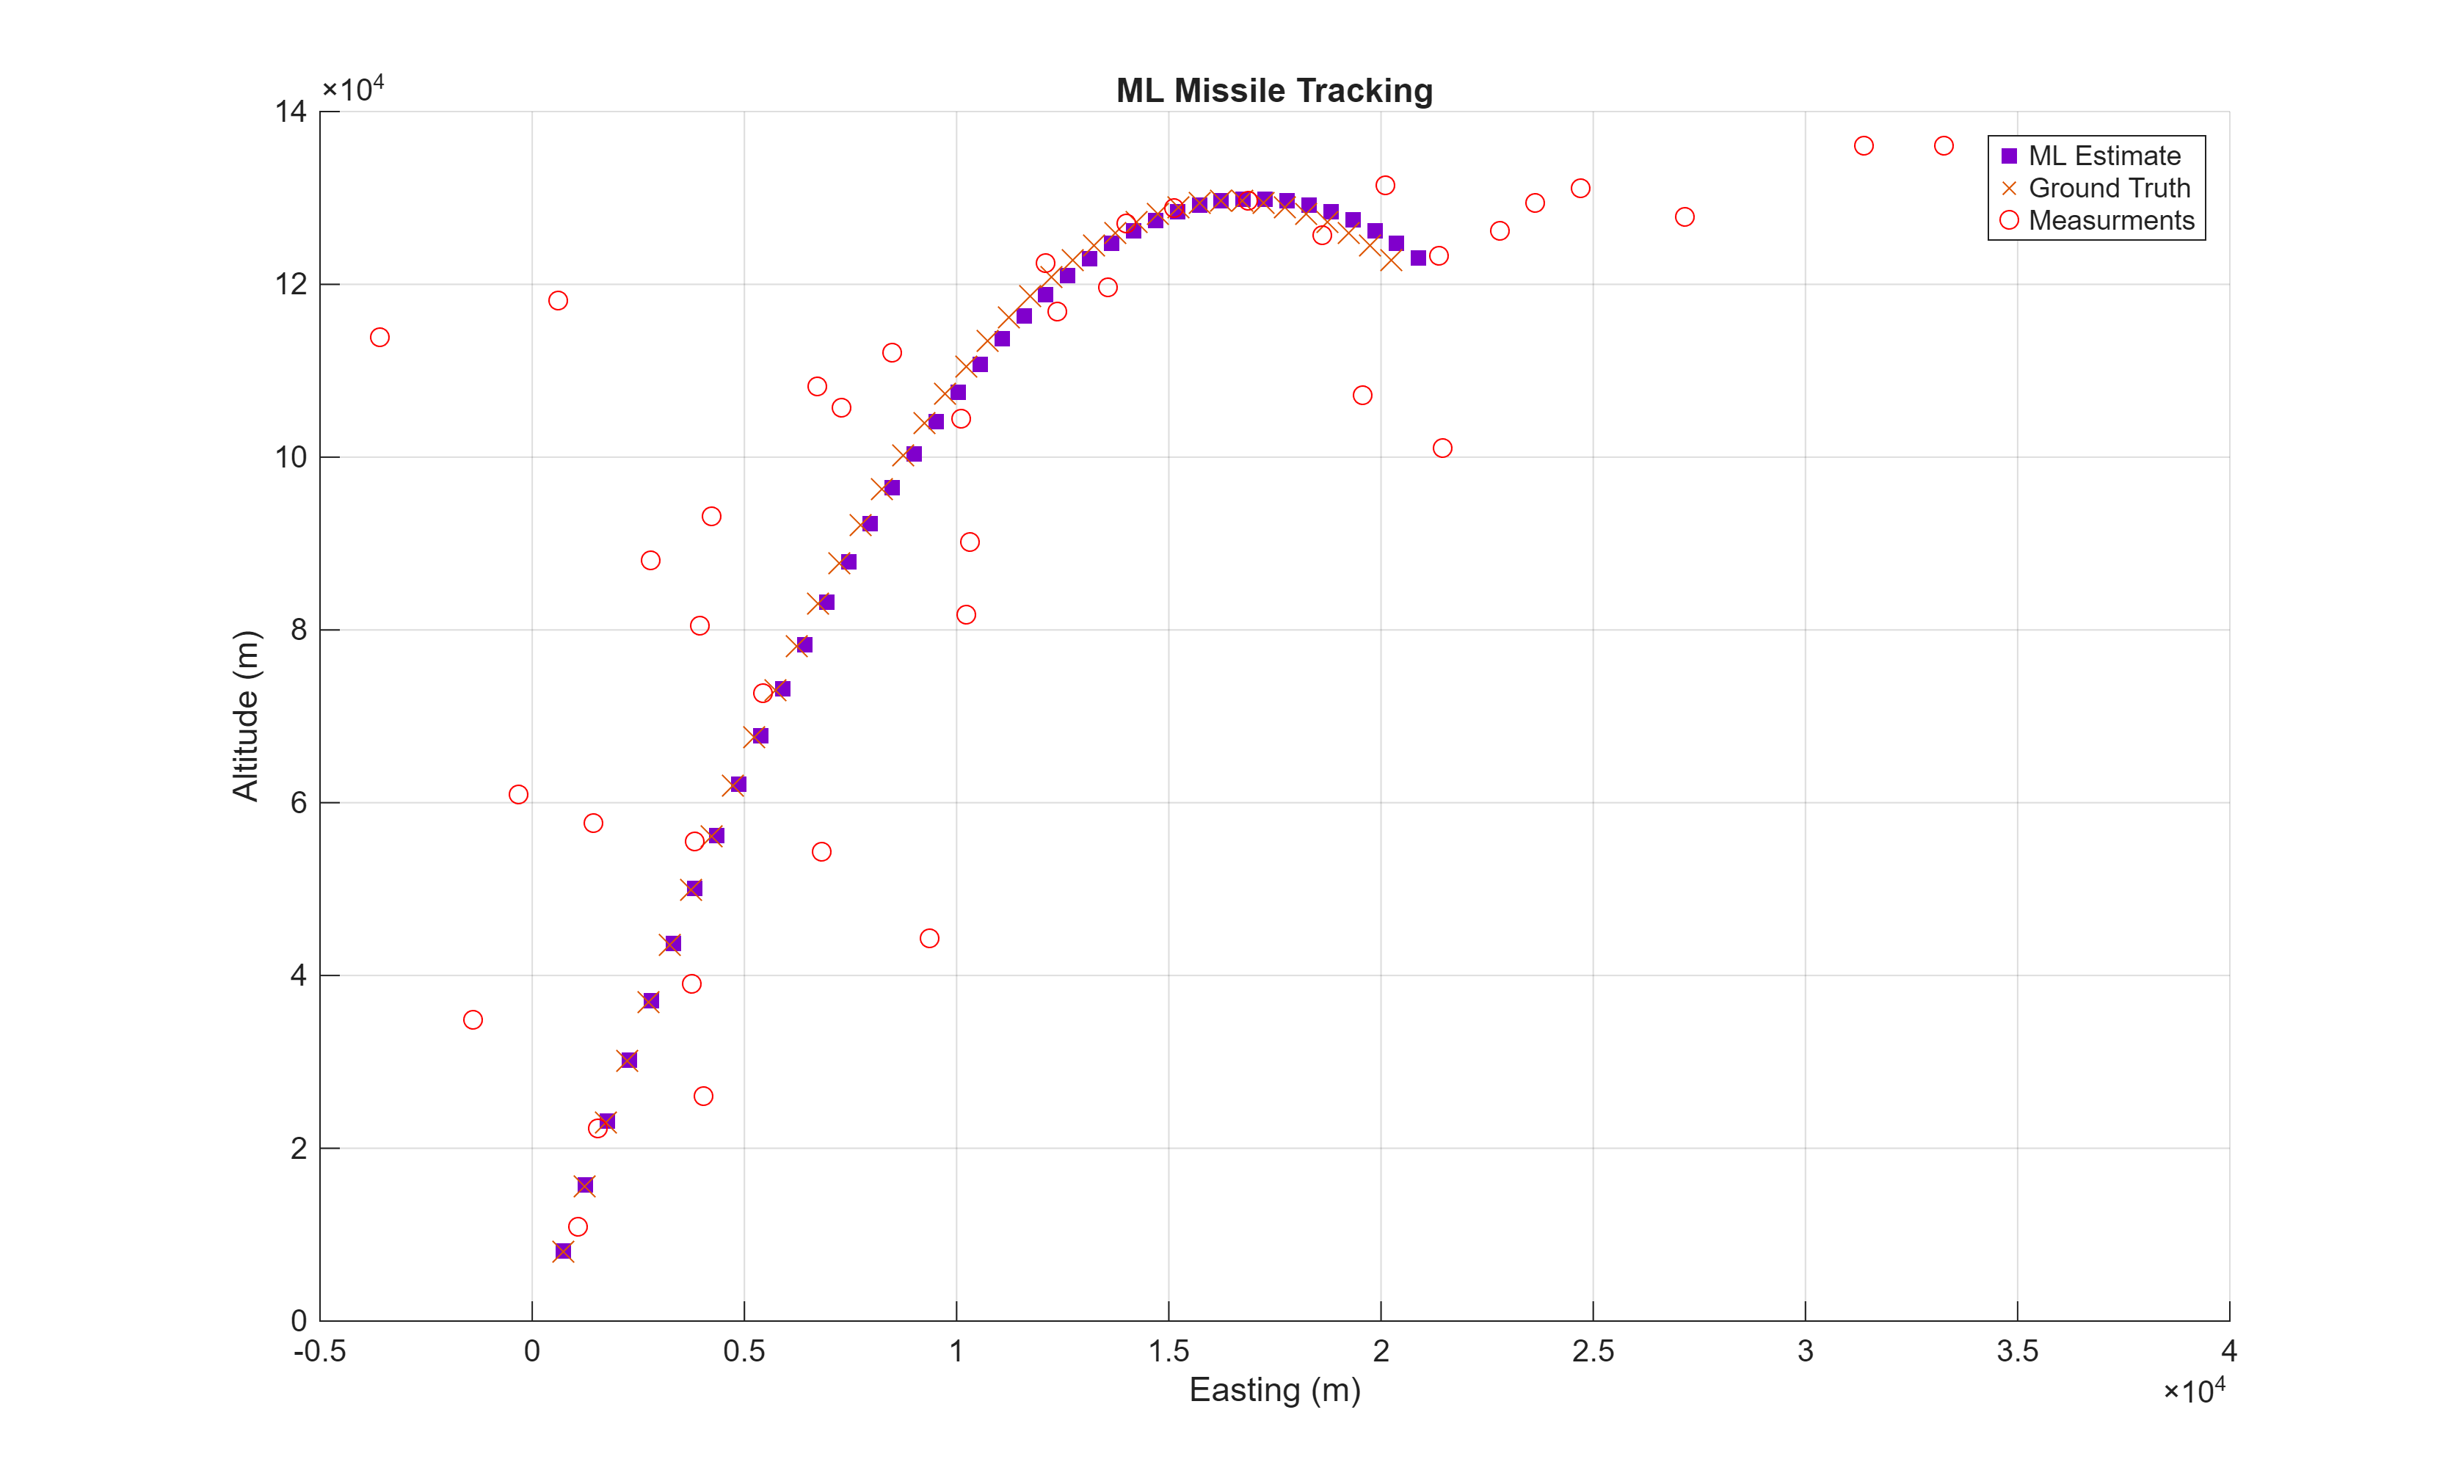
\includegraphics[width=\textwidth, height=0.75\textheight, keepaspectratio]{Figures/ML_estimate.png}
        \caption{Maximum Likelihood Estimated Trajectory}
    \label{fig:ML}
    \end{figure}

    \begin{figure}[h]
        \centering
        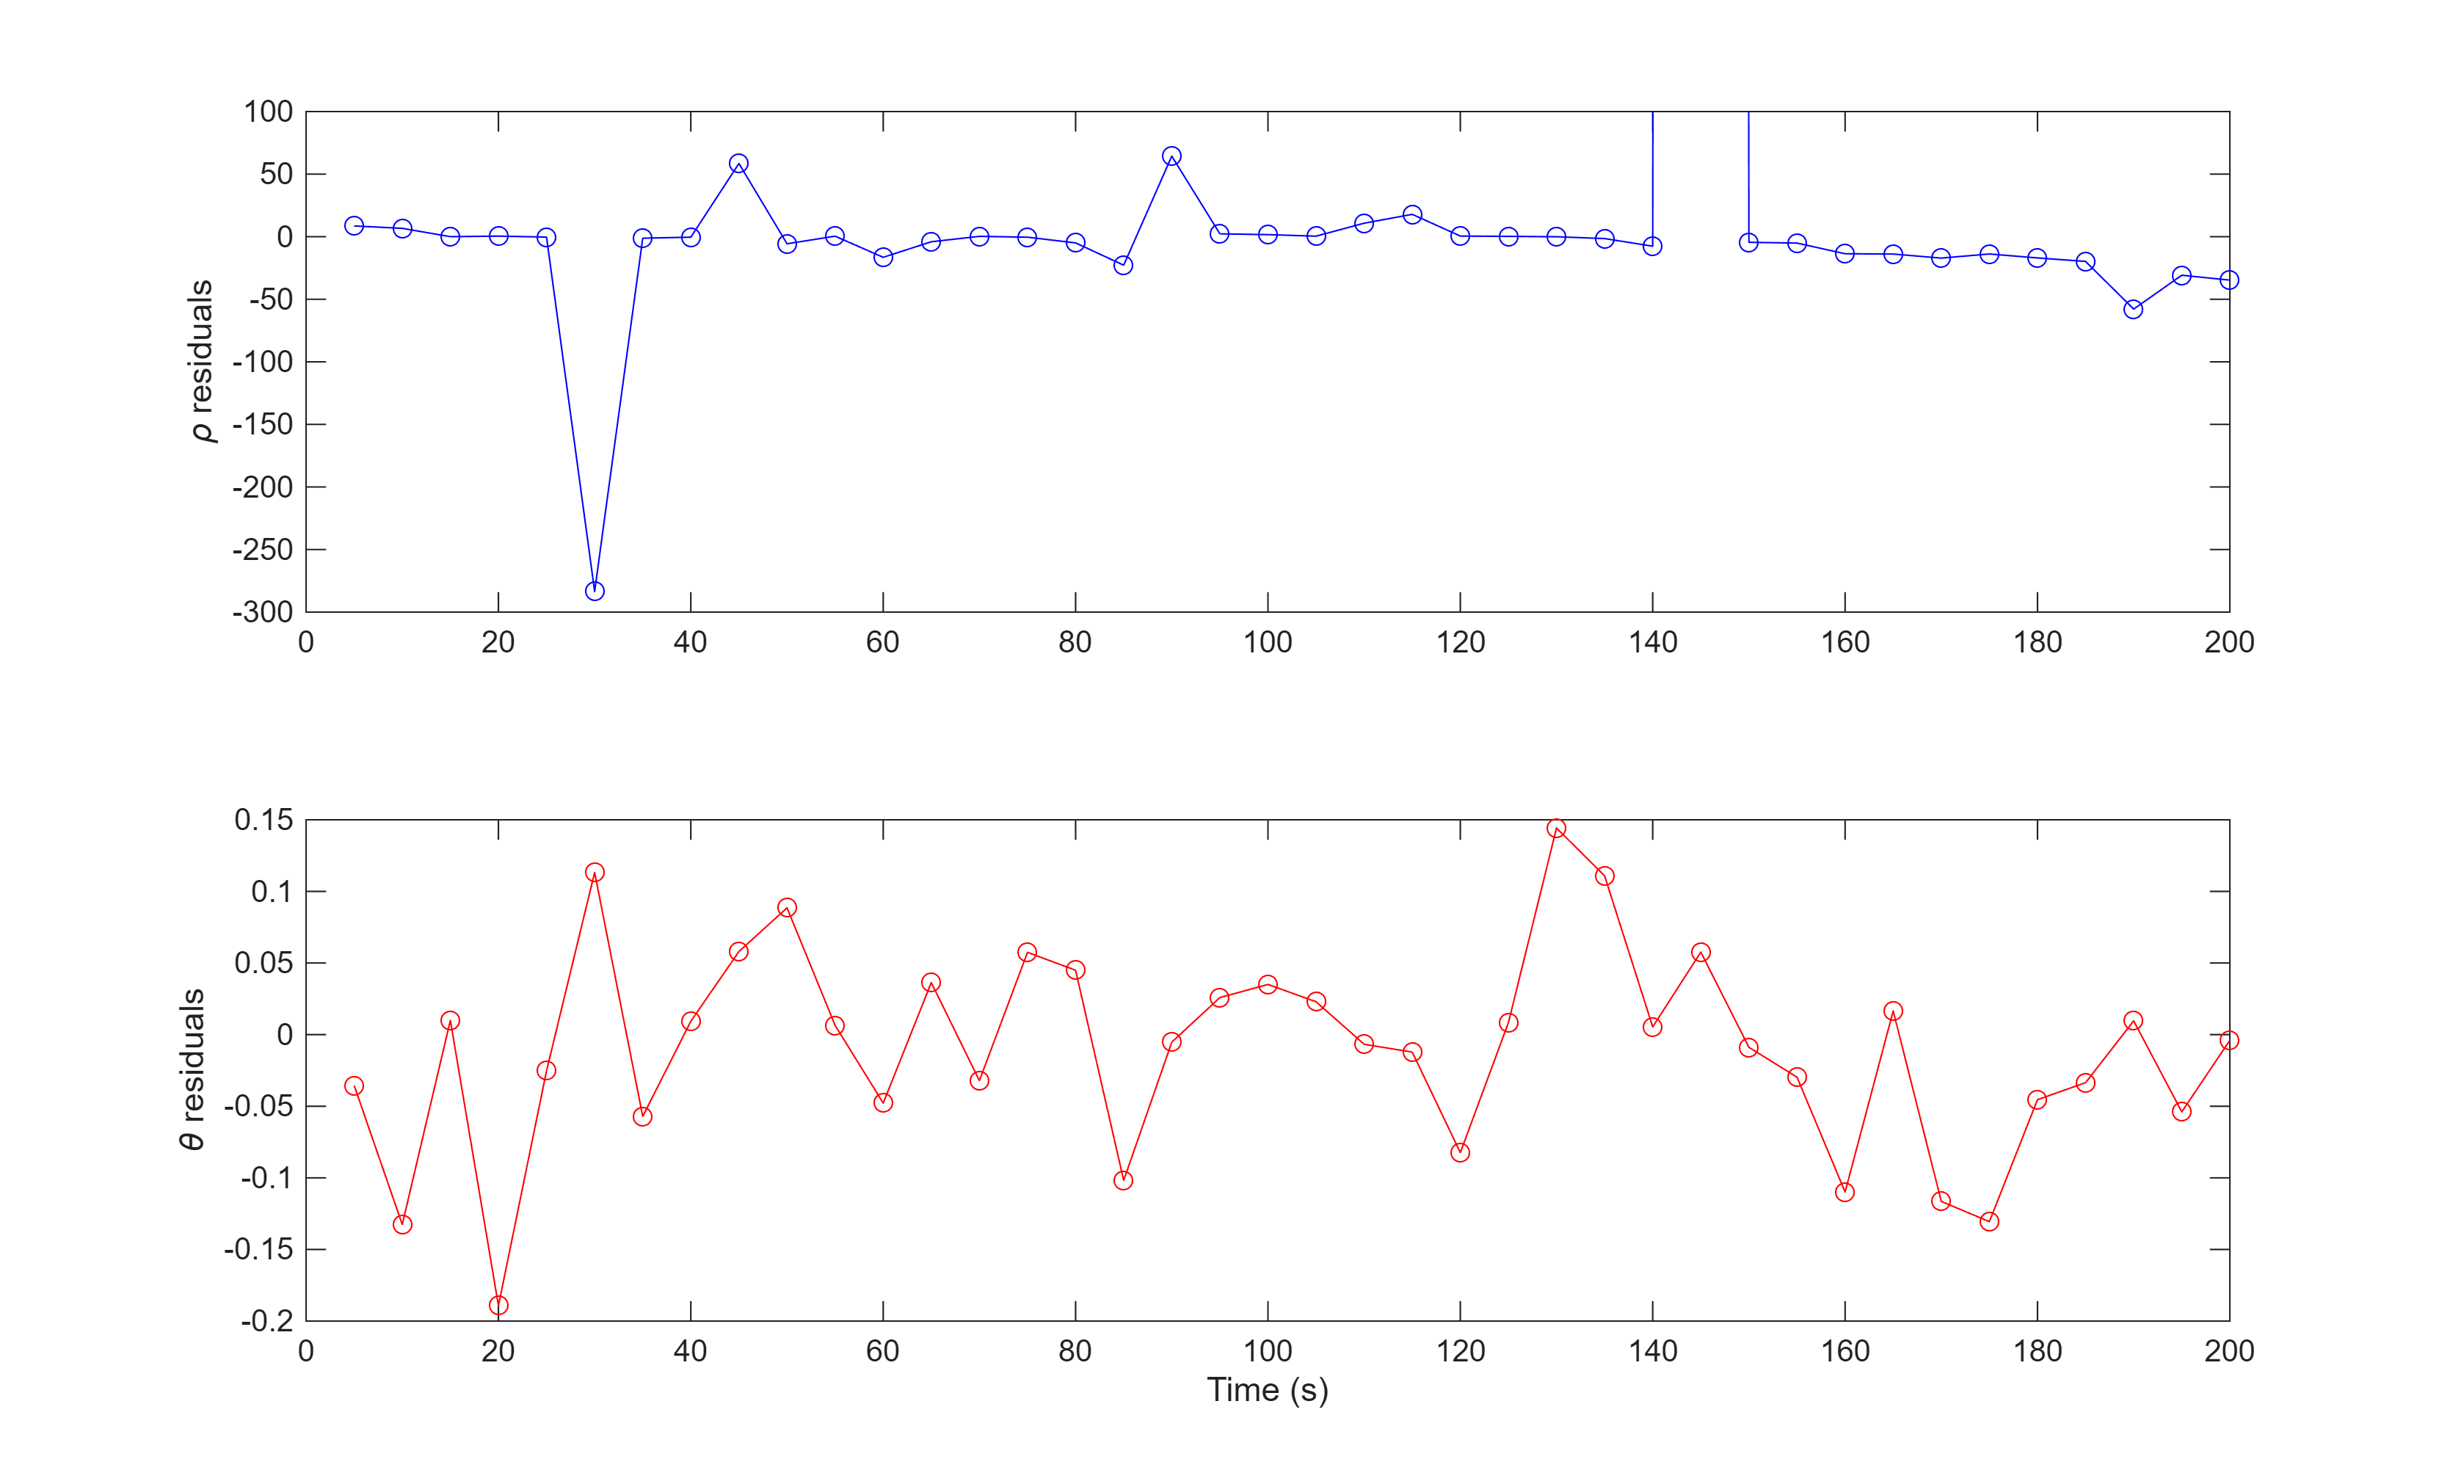
\includegraphics[width=\textwidth, height=0.75\textheight, keepaspectratio]{Figures/ML_estimate_Res.png}
        \caption{Maximum Likelihood Residuals with $\rho$ Outlier Removed}
    \label{fig:MLRes}
    \end{figure}

    After some trial and error, I was able to land on an initial $x_0 = [50 \ 300 \ 20 \ 100]^T$ resulting in an estimate of 
    $\hat{x}_{0,ML} = [220.5 \ 103.3 \ 294.3 \ 1.6 \times 10^3]^T$. To do this, I used MATLAB's \texttt{fminunc} function, and I specified my own gradient vector specified in equation (\ref{eq:finalGrad}). I found it difficult to land on a good estimate for
    $x_0$ without specifying a gradient, and I found MATLAB's \texttt{checkGradients} function to be quite helpful in debugging. As expected, maximum likelihood performs much better than NLS as seen in figure \ref{fig:ML}.
    \newpage
    \item
    
    Comparing the results of part (e) to part (b), we see that the range residuals from ML are significantly smaller than that of NLS as seen in figure \ref{fig:MLRes}. The bearing residuals are more or less the same. Since the bearing noise is gaussian,
    makes sense that NLS would be able to resolve a good bearing estimate from the given data set.
    In terms of error, the error from the ML estimate was $[13.53 \ -3.33 \ -125.3 \ -0.76]^T$, which is orders of magnitude smaller than that of NLS. If we wanted to go about finding the bias and covariance of $\hat{x}_{0,ML}$, we would have a few options.
    If it is possible to find an analytic expression for $\hat{x}_{0,ML}$, we could use the following expressions, 
    \[
     \mathrm{Bias} = \mathbb{E}[\hat{x}_{0,ML}] - x_0 \quad \Cov(\hat{x}_{0,ML}) = \mathbb{E}[(\tilde{x}_0 - \bar{\tilde{x}}_0)(...)^t]
    \]
    Where $\tilde{x}_0 = x_0 - \hat{x}_{0,ML}$ and $\bar{\tilde{x}}_0 = \mathbb{E}[\tilde{x}_0]$. However, due to the dimensionality of the problem and highly non-linear measurement and noise model, finding an analytical expression for $\hat{x}_{0,ML}$
    is unlikely. Instead, we could estimate the bias and covariance using Monte Carlo trials. We can fix a value for $x_0$ and sample $N$ measurements from $P(y\mid x_0)$ for each $m = 1,2 \cdots M$ MC trial. $\mathbb{E}[\hat{x}_{0,ML}]$ and $\mathbb{E}[\bar{\tilde{x}}_{0}]$ can then be estimated using the values of $\hat{x}_{0,ML}$
    \texttt{fminunc} converges to across each MC trial.
\end{enumerate}

\lstdefinestyle{matlab}{
  language=Matlab,
  basicstyle=\ttfamily\small,
  numbers=left,
  numberstyle=\tiny,
  stepnumber=1,
  numbersep=8pt,
  showstringspaces=false,
  breaklines=true,
  breakatwhitespace=true,
  tabsize=4,
  frame=single,
  captionpos=b
}
\newpage

\subsection{Code for Problem 3a}
\begin{lstlisting}[style = matlab]
%%% Bijan Jourabchi
%%% ASEN 6044 HW2 Q3a

%%% Load Datafile
clear; clc; close all
load("homework1_missileprob_data.mat")
ystackedOG = ystacked;
x0trueOG = x0true;
load("hw2_missileprob_data.mat")

N = size(ystacked,1)/2;
np = 2;
L = 80000;
dt = 5; % sec
t = dt:dt:N*dt;

% Get measurment in x,y coords
rho = ystacked(1:2:end);
theta = ystacked(2:2:end);

rhoOG = ystackedOG(1:2:end);
thetaOG = ystackedOG(2:2:end);


for i = 1:N
    aM_1(i) = rho(i)*sin(theta(i));
    eM_1(i) = L - rho(i)*cos(theta(i));

    aM_2(i) = rhoOG(i)*sin(thetaOG(i));
    eM_2(i) = L - rhoOG(i)*cos(thetaOG(i));
    % Get trajectories
    [eT_1(i),aT_1(i)] = f(x0trueOG,t(i));
    [eT_2(i),aT_2(i)] = f(x0trueOG,t(i));

end

figure(); hold on; grid on

scatter(eM_1,aM_1,'ro')
scatter(eM_2,aM_2,'bo')
scatter(eT_2,aT_2,'kx')
xlabel('\zeta (m)')
ylabel('a (m)')

legend('Original Noise Model','New Noise Model','Trajectory',Location='southeast')
% Create Figures folder if it doesn't exist and save the current figure
figDir = fullfile(pwd,'Figures');
if ~exist(figDir,'dir')
    mkdir(figDir);
end

% Prepare filename with timestamp to avoid overwriting
timestamp = datestr(now,'yyyy-mm-dd_HHMMSS');
fname = fullfile(figDir,['missile_measurments' '.png']);

% Set figure properties for saving
fig = gcf;
set(fig,'Color','w','PaperPositionMode','auto');

% Save as PNG (use -r300 for high resolution)
print(fig,'-dpng','-r300',fname);

function [xik,ak] = f(x0,t)

    xi0 = x0(1);
    xid0 = x0(2);
    a0 = x0(3);
    ad0 = x0(4);
    g = 9.81;

    xik = xi0 + xid0*t;
    ak = a0 + ad0*t - 0.5*g*t^2;
end
\end{lstlisting}
\subsection{Code for Problem 3b}
\begin{lstlisting}[style=matlab]
%%% Bijan Jourabchi
%%% ASEN 6044 HW2 Q3

%%% Load Datafile
clear; clc; close all
load("hw2_missileprob_data.mat")

%%% Get Noise Covar matrix

N = size(ystacked,1)/2;
np = 2;
L = 80000;
dt = 5; % sec
t = dt:dt:N*dt;

R = [70 0; 0 0.005];
Rb = kron(eye(N), R);

%%% Whitening transformation

S = chol(Rb);
ya = S*ystacked;

%%% NLS
x0g = [10;30;230;100];
%x0g = [235;-150;200;2000];
%x0g = x0true;

% NLS
itr = 0;
maxitr = 100;
maxalph = 10;
converged = false;

while itr < maxitr && ~converged
    % Setup NLS
    yc = zeros(np,N);
    H = zeros(np*N,4);
    
    for k = 1:N
    
        yc(:,k) = h(x0g,t(k),R, L,true);
    
        %[xi,a] = f(x0g,t(k));
        H(2*k-1 : 2*k, :) = jcb(x0g,L,t(k));
    end
    yc = S*yc(:);
    H = S*H;

    % Cost fxn
    
    residuals = ya - yc;
    Jcurr = residuals'/Rb*residuals;
    dx = inv(H'*inv(Rb)*H)*H'*inv(Rb)*(ya - yc);
    alph = 1;
    alphsplts = 0;
    while alphsplts < maxalph

        xn0 = x0g + alph*dx;
        
        

        yc = zeros(np,N);
        for k = 1:N
            yc(:,k) = h(xn0,t(k),R, L,true);
        end
        yc = S*yc(:);

        Jn = (ya - yc)'/Rb*(ya - yc);

        if abs(Jcurr - Jn) < 50
            converged = true;
            break;
        end

        if Jn > Jcurr
            alph = alph/2;
        else
            x0g = xn0;
            break;
        end
        alphsplts = alphsplts + 1;
    end
    itr = itr + 1;
end

err = x0true - x0g %% ERROR

for k = 1:N

        H(2*k-1 : 2*k, :) = jcb(x0g,80000,t(k));
end

P = inv(H'*inv(Rb)*H);
plot_NLS(x0true,x0g,ystacked,t,Rb,L)


%%% Measurment function
function [y] = h(x0,t,R,L,noise)

    if noise
        vk = mvnrnd([0,0],R)';
    else 
        vk = [0 0];
    end

    [xik,ak] = f(x0,t);

    rho = sqrt((L - xik)^2 + ak^2) + vk(1);
    theta = atan2(ak,(L-xik)) + vk(2);

    y = [rho;theta];
end

%%% Dynamics function
function [xik,ak] = f(x0,t)

    xi0 = x0(1);
    xid0 = x0(2);
    a0 = x0(3);
    ad0 = x0(4);
    g = 9.81;

    xik = xi0 + xid0*t;
    ak = a0 + ad0*t - 0.5*g*t^2;
end

%%% Jacobian fxn 
function [H] = jcb(x,L,t)
    
    xi = x(1);
    xid = x(2);
    a = x(3);
    ad = x(4);
    g = 9.81;

    H11 = 2*(xid*t+xi-L)/sqrt((2*a-g*t^2+2*ad*t)^2 + 4*(xid*t+xi-L)^2);
    H12 = H11 * t;
    H13 = (2*a - g*t^2 + 2*ad*t) / sqrt((2*a-g*t^2+2*ad*t)^2 + 4*(xid*t+xi-L)^2);
    H14 = H13*t;

    H21 = 2*(2*a - g*t^2 + 2*ad*t)/((2*a - g*t^2 +2*ad*t)^2 + 4*(xid*t+xi-L)^2);
    H22 = H21*t;
    H23 = 4*(-xid*t-xi+L)/((2*a - g*t^2 +2*ad*t)^2 + 4*(xid*t+xi-L)^2);
    H24 = -t*H23;

    H = [H11 H12 H13 H14;H21 H22 H23 H24];
end

%%% Plotting Functions
function [] = plot_NLS(x0t,x0NLS,Y,tvec,R,L)
    
    N = length(tvec);

    % Get Truth/Estimated Traj

    trajT = zeros(2,N);
    trajE = zeros(2,N);
    
    
    for k = 1:N
        [xi,a] = f(x0t,tvec(k));
        trajT(:,k) = [xi;a];
        [xi,a] = f(x0NLS,tvec(k));
        trajE(:,k) = [xi;a];
    end

    % Get measurment in x,y coords
    rho = Y(1:2:end);
    theta = Y(2:2:end);
    for i = 1:N
        aM(i) = rho(i)*sin(theta(i));
        eM(i) = L - rho(i)*cos(theta(i));

        y_est = h(x0NLS,tvec(i),eye(2),L,false);
        rho_est(i) = y_est(1);
        theta_est(i) = y_est(2);
    end

    
    figure(4); hold on; grid on
    scatter(trajE(1,:),trajE(2,:), 's', 'MarkerFaceColor', [0.5 0 0.8], 'MarkerEdgeColor', [0.5 0 0.8])
    scatter(trajT(1,:),trajT(2,:),100,'x','Color', '#40E0D0')
    scatter(eM,aM,'ro')
    legend('NLS Estimate','Ground Truth','Measurments')
    xlabel("Easting (m)")
    ylabel("Altitude (m)")
    title("NLS Missile Tracking")

    fname = fullfile('Figures',['NLS_estimate' '.png']);

    % Set figure properties for saving
    fig = gcf;
    set(fig,'Color','w','PaperPositionMode','auto');
    
    % Save as PNG (use -r300 for high resolution)
    print(fig,'-dpng','-r300',fname);

     % Residual Plot
    figure(6); hold on; grid on
    tiledlayout(2,1)
    nexttile;
    plot(tvec,rho_est(:) - rho,'-o','Color','b')
    ylabel('\rho residuals')
    ylim([-2500 1500])
    nexttile;
    plot(tvec,theta_est(:) - theta,'-o','Color','r')
    xlabel("Time (s)")
    ylabel("\theta residuals")

    fname = fullfile('Figures',['NLS_estimate_Res' '.png']);

    % Set figure properties for saving
    fig = gcf;
    set(fig,'Color','w','PaperPositionMode','auto');
    
    % Save as PNG (use -r300 for high resolution)
    print(fig,'-dpng','-r300',fname);

    figure(67); hold on; grid on
    plot(tvec,rho_est(:) - rho,'-o','Color','b')
    ylabel('\rho residuals')
    xlabel("Time (s)")
    ylim([-2500 1500])

    fname = fullfile('Figures',['NLS_Rho_Res' '.png']);

    % Set figure properties for saving
    fig = gcf;
    set(fig,'Color','w','PaperPositionMode','auto');
    
    % Save as PNG (use -r300 for high resolution)
    print(fig,'-dpng','-r300',fname);
    

end

\end{lstlisting}
\subsection{Code for Problem 3e}
\begin{lstlisting}[style=matlab]
%%% ASEN 6044 HW2 Q3e

%%% Load Datafile
clear; clc; close all
load("hw2_missileprob_data.mat")

%%% Constants
N = size(ystacked,1)/2;
np = 2;
L = 80000;
dt = 5; % sec
t = dt:dt:N*dt;

fun = @(x) Liklihood(x, ystacked,t);
options = optimoptions('fminunc','Algorithm','trust-region','SpecifyObjectiveGradient',true,'MaxFunctionEvaluations', 30000, 'MaxIterations', 10000);

x0 = [50;300;20;100];

[x,fval] = fminunc(fun,x0,options);


%%% Plot Results
err = x0true - x %% ERROR
results(x0true,x,ystacked,t,L)

function [Like,G] = Liklihood(x,Y,t)

% Unpack
xi = x(1);
xid = x(2);
a = x(3);
ad = x(4);
rho = Y(1:2:end);
theta = Y(2:2:end);

% Constants
nu = 1/2;
sigma2 = 0.005;
L = 80000;
g = 9.81;

% Dynamics
xit = xi + xid*t;
at = a+ad*t-0.5*g*t.^2;

% Force col vector
xit = xit(:);
at = at(:);

% P(rho_k|x0)

% Constant terms
C = gamma(((nu+1)/2))/gamma(nu/2) * (1/(sqrt(nu*pi)));

Pr = C*((1 + ((rho - sqrt((L - xit).^2+(at).^2)).^2)/nu)).^(-(nu+1)/2);

% P(theta_k|x0)

% Constant term
C = 1/(sqrt(sigma2*2*pi));

Pb = C*exp((-(theta-atan2(at,(L-xit))).^2)/(2*sigma2));

Like = -sum(log(Pr.*Pb));

%% Gradient Vector
if nargout > 1
    t = t(:);
    % First Vector
    C1 = (nu+1)/2;

    G11 = (2*(rho - sqrt((L - xit).^2+(at).^2)).*(L-xit))./((((rho - sqrt((L - xit).^2+(at).^2)).^2) + nu).*(sqrt((L - xit).^2+(at).^2)));
    G12 = G11.*t;
    G13 = (-2*(rho - sqrt((L - xit).^2+(at).^2)).*at)./((((rho - sqrt((L - xit).^2+(at).^2)).^2) + nu).*(sqrt((L - xit).^2+(at).^2)));
    G14 = G13.*t;

    G11 = sum(G11);
    G12 = sum(G12);
    G13 = sum(G13);
    G14 = sum(G14);

    C2 = 1/(2*sigma2);
    G21 = (-2*(theta-atan2(at,(L-xit))).*at)./(((at./(L-xit)).^2 + 1).*(L-xit).^2);
    G22 = G21.*t;
    G23 = (-2*(theta-atan2(at,(L-xit))))./(((at./(L-xit)).^2 + 1).*(L-xit));
    G24 = G23.*t;

    G21 = sum(G21);
    G22 = sum(G22);
    G23 = sum(G23);
    G24 = sum(G24);

    G = C1*[G11;G12;G13;G14]+ C2*[G21;G22;G23;G24];
end
end

%%% Plotting Functions
function [] = results(x0t,x0_hat,Y,tvec,L)

    N = length(tvec);

    % Get Truth/Estimated Traj

    trajT = zeros(2,N);
    trajE = zeros(2,N);
    
    
    for k = 1:N
        [xi,a] = f(x0t,tvec(k));
        trajT(:,k) = [xi;a];
        [xi,a] = f(x0_hat,tvec(k));
        trajE(:,k) = [xi;a];
    end
    
    rho = Y(1:2:end);
    theta = Y(2:2:end);
    % Get measurment in x,y coords
    for i = 1:N
        aM(i) = rho(i)*sin(theta(i));
        eM(i) = L - rho(i)*cos(theta(i));

        y_est = h(x0_hat,tvec(i),L);
        rho_est(i) = y_est(1);
        theta_est(i) = y_est(2);
    end

    
    figure(2); hold on; grid on
    scatter(trajE(1,:),trajE(2,:), 's', 'MarkerFaceColor', [0.5 0 0.8], 'MarkerEdgeColor', [0.5 0 0.8])
    scatter(trajT(1,:),trajT(2,:),100,'x','Color', '#40E0D0')
    scatter(eM,aM,'ro')
    legend('ML Estimate','Ground Truth','Measurments')
    xlabel("Easting (m)")
    ylabel("Altitude (m)")
    title("ML Missile Tracking")

    fname = fullfile('Figures',['ML_estimate' '.png']);

    % Set figure properties for saving
    fig = gcf;
    set(fig,'Color','w','PaperPositionMode','auto');
    
    % Save as PNG (use -r300 for high resolution)
    print(fig,'-dpng','-r300',fname);
    
    % Residual Plot
    figure(3); hold on; grid on
    tiledlayout(2,1)
    nexttile;
    plot(tvec,rho_est(:) - rho,'-o','Color','b')
    ylabel('\rho residuals')
    ylim([-300 100])

    nexttile;
    plot(tvec,theta_est(:) - theta,'-o','Color','r')
    xlabel("Time (s)")
    ylabel("\theta residuals")

    fname = fullfile('Figures',['ML_estimate_Res' '.png']);

    % Set figure properties for saving
    fig = gcf;
    set(fig,'Color','w','PaperPositionMode','auto');
    
    % Save as PNG (use -r300 for high resolution)
    print(fig,'-dpng','-r300',fname);

    figure(67); hold on; grid on
    plot(tvec,rho_est(:) - rho,'-o','Color','b')
    ylabel('\rho residuals')
    xlabel("Time (s)")
    ylim([-300 100])

    fname = fullfile('Figures',['ML_Rho_Res' '.png']);

    % Set figure properties for saving
    fig = gcf;
    set(fig,'Color','w','PaperPositionMode','auto');
    
    % Save as PNG (use -r300 for high resolution)
    print(fig,'-dpng','-r300',fname);
    

end

function [y] = h(x0,t, L)

    
    vk = [0 0];

    [xik,ak] = f(x0,t);

    rho = sqrt((L - xik)^2 + ak^2) + vk(1);
    theta = atan2(ak,(L-xik)) + vk(2);

    y = [rho;theta];
end

%%% Dynamics function
function [xik,ak] = f(x0,t)

    xi0 = x0(1);
    xid0 = x0(2);
    a0 = x0(3);
    ad0 = x0(4);

    g = 9.81;

    xik = xi0 + xid0*t;
    ak = a0 + ad0*t - 0.5*g*t^2;
end
\end{lstlisting}
% =====================================================

\end{document}
